% Options for packages loaded elsewhere
\PassOptionsToPackage{unicode}{hyperref}
\PassOptionsToPackage{hyphens}{url}
%


\PassOptionsToPackage{table}{xcolor}

\documentclass[
  10pt,
  letterpaper,
]{article}

\usepackage{amsmath,amssymb}
\usepackage{iftex}
\ifPDFTeX
  \usepackage[T1]{fontenc}
  \usepackage[utf8]{inputenc}
  \usepackage{textcomp} % provide euro and other symbols
\else % if luatex or xetex
  \usepackage{unicode-math}
  \defaultfontfeatures{Scale=MatchLowercase}
  \defaultfontfeatures[\rmfamily]{Ligatures=TeX,Scale=1}
\fi
\usepackage{lmodern}
\ifPDFTeX\else  
    % xetex/luatex font selection
\fi
% Use upquote if available, for straight quotes in verbatim environments
\IfFileExists{upquote.sty}{\usepackage{upquote}}{}
\IfFileExists{microtype.sty}{% use microtype if available
  \usepackage[]{microtype}
  \UseMicrotypeSet[protrusion]{basicmath} % disable protrusion for tt fonts
}{}
\makeatletter
\@ifundefined{KOMAClassName}{% if non-KOMA class
  \IfFileExists{parskip.sty}{%
    \usepackage{parskip}
  }{% else
    \setlength{\parindent}{0pt}
    \setlength{\parskip}{6pt plus 2pt minus 1pt}}
}{% if KOMA class
  \KOMAoptions{parskip=half}}
\makeatother
\usepackage{xcolor}
\usepackage[top=0.85in,left=2.75in,footskip=0.75in]{geometry}
\setlength{\emergencystretch}{3em} % prevent overfull lines
\setcounter{secnumdepth}{-\maxdimen} % remove section numbering


\providecommand{\tightlist}{%
  \setlength{\itemsep}{0pt}\setlength{\parskip}{0pt}}\usepackage{longtable,booktabs,array}
\usepackage{calc} % for calculating minipage widths
% Correct order of tables after \paragraph or \subparagraph
\usepackage{etoolbox}
\makeatletter
\patchcmd\longtable{\par}{\if@noskipsec\mbox{}\fi\par}{}{}
\makeatother
% Allow footnotes in longtable head/foot
\IfFileExists{footnotehyper.sty}{\usepackage{footnotehyper}}{\usepackage{footnote}}
\makesavenoteenv{longtable}
\usepackage{graphicx}
\makeatletter
\def\maxwidth{\ifdim\Gin@nat@width>\linewidth\linewidth\else\Gin@nat@width\fi}
\def\maxheight{\ifdim\Gin@nat@height>\textheight\textheight\else\Gin@nat@height\fi}
\makeatother
% Scale images if necessary, so that they will not overflow the page
% margins by default, and it is still possible to overwrite the defaults
% using explicit options in \includegraphics[width, height, ...]{}
\setkeys{Gin}{width=\maxwidth,height=\maxheight,keepaspectratio}
% Set default figure placement to htbp
\makeatletter
\def\fps@figure{htbp}
\makeatother

% Use adjustwidth environment to exceed column width (see example table in text)
\usepackage{changepage}

% marvosym package for additional characters
\usepackage{marvosym}

% cite package, to clean up citations in the main text. Do not remove.
% Using natbib instead
% \usepackage{cite}

% Use nameref to cite supporting information files (see Supporting Information section for more info)
\usepackage{nameref,hyperref}

% line numbers
\usepackage[right]{lineno}

% ligatures disabled
\usepackage{microtype}
\DisableLigatures[f]{encoding = *, family = * }

% create "+" rule type for thick vertical lines
\newcolumntype{+}{!{\vrule width 2pt}}

% create \thickcline for thick horizontal lines of variable length
\newlength\savedwidth
\newcommand\thickcline[1]{%
  \noalign{\global\savedwidth\arrayrulewidth\global\arrayrulewidth 2pt}%
  \cline{#1}%
  \noalign{\vskip\arrayrulewidth}%
  \noalign{\global\arrayrulewidth\savedwidth}%
}

% \thickhline command for thick horizontal lines that span the table
\newcommand\thickhline{\noalign{\global\savedwidth\arrayrulewidth\global\arrayrulewidth 2pt}%
\hline
\noalign{\global\arrayrulewidth\savedwidth}}

% Text layout
\raggedright
\setlength{\parindent}{0.5cm}
\textwidth 5.25in 
\textheight 8.75in

% Bold the 'Figure #' in the caption and separate it from the title/caption with a period
% Captions will be left justified
\usepackage[aboveskip=1pt,labelfont=bf,labelsep=period,justification=raggedright,singlelinecheck=off]{caption}
\renewcommand{\figurename}{Fig}

% Remove brackets from numbering in List of References
\makeatletter
\renewcommand{\@biblabel}[1]{\quad#1.}
\makeatother

% Header and Footer with logo
\usepackage{lastpage,fancyhdr}
\usepackage{epstopdf}
%\pagestyle{myheadings}
\pagestyle{fancy}
\fancyhf{}
%\setlength{\headheight}{27.023pt}
%\lhead{\includegraphics[width=2.0in]{PLOS-submission.eps}}
\rfoot{\thepage/\pageref{LastPage}}
\renewcommand{\headrulewidth}{0pt}
\renewcommand{\footrule}{\hrule height 2pt \vspace{2mm}}
\fancyheadoffset[L]{2.25in}
\fancyfootoffset[L]{2.25in}
\lfoot{\today}
\usepackage{booktabs}
\usepackage{caption}
\usepackage{longtable}
\usepackage{colortbl}
\usepackage{array}
\usepackage{anyfontsize}
\usepackage{multirow}
\usepackage{float}
\floatplacement{table}{H}
\floatplacement{figure}{H}
\usepackage{pdflscape}
\newcommand{\blandscape}{\begin{landscape}}
\newcommand{\elandscape}{\end{landscape}}
\makeatletter
\@ifpackageloaded{caption}{}{\usepackage{caption}}
\AtBeginDocument{%
\ifdefined\contentsname
  \renewcommand*\contentsname{Table of contents}
\else
  \newcommand\contentsname{Table of contents}
\fi
\ifdefined\listfigurename
  \renewcommand*\listfigurename{List of Figures}
\else
  \newcommand\listfigurename{List of Figures}
\fi
\ifdefined\listtablename
  \renewcommand*\listtablename{List of Tables}
\else
  \newcommand\listtablename{List of Tables}
\fi
\ifdefined\figurename
  \renewcommand*\figurename{Figure}
\else
  \newcommand\figurename{Figure}
\fi
\ifdefined\tablename
  \renewcommand*\tablename{Table}
\else
  \newcommand\tablename{Table}
\fi
}
\@ifpackageloaded{float}{}{\usepackage{float}}
\floatstyle{ruled}
\@ifundefined{c@chapter}{\newfloat{codelisting}{h}{lop}}{\newfloat{codelisting}{h}{lop}[chapter]}
\floatname{codelisting}{Listing}
\newcommand*\listoflistings{\listof{codelisting}{List of Listings}}
\makeatother
\makeatletter
\makeatother
\makeatletter
\@ifpackageloaded{caption}{}{\usepackage{caption}}
\@ifpackageloaded{subcaption}{}{\usepackage{subcaption}}
\makeatother
\ifLuaTeX
  \usepackage{selnolig}  % disable illegal ligatures
\fi
\usepackage[numbers,square,comma]{natbib}
\bibliographystyle{plos2015}
\usepackage{bookmark}

\IfFileExists{xurl.sty}{\usepackage{xurl}}{} % add URL line breaks if available
\urlstyle{same} % disable monospaced font for URLs
\hypersetup{
  pdftitle={A family of accessibility measures derived from spatial interaction principles},
  pdfauthor={Anastasia Soukhov; Rafael H. M. Pereira; Christopher D. Higgins; Antonio Páez},
  hidelinks,
  pdfcreator={LaTeX via pandoc}}



\begin{document}
\vspace*{0.2in}

% Title must be 250 characters or less.
\begin{flushleft}
{\Large
\textbf\newline{A family of accessibility measures derived from spatial
interaction
principles} % Please use "sentence case" for title and headings (capitalize only the first word in a title (or heading), the first word in a subtitle (or subheading), and any proper nouns).
}
\newline
\\
% Insert author names, affiliations and corresponding author email (do not include titles, positions, or degrees).
Anastasia Soukhov\textsuperscript{1}, Rafael H. M.
Pereira\textsuperscript{2}, Christopher D.
Higgins\textsuperscript{3*}, Antonio Páez\textsuperscript{1}
\\
\bigskip
\textbf{1} McMaster University, School of Earth, Environment \&
Society, Hamilton, Canada, \\ \textbf{2} Institute for Applied Economic
Research - Ipea, Data Science Division, Brasília,
Brazil, \\ \textbf{3} University of Toronto Scarborough, Department of
Human Geography, Toronto, Canada, 
\bigskip

% Insert additional author notes using the symbols described below. Insert symbol callouts after author names as necessary.
% 
% Remove or comment out the author notes below if they aren't used.
%
% Primary Equal Contribution Note
\Yinyang These authors contributed equally to this work.

% Additional Equal Contribution Note
% Also use this double-dagger symbol for special authorship notes, such as senior authorship.
%\ddag These authors also contributed equally to this work.

% Current address notes
\textcurrency Current Address: Dept/Program/Center, Institution Name, City, State, Country % change symbol to "\textcurrency a" if more than one current address note
% \textcurrency b Insert second current address 
% \textcurrency c Insert third current address

% Deceased author note
\dag Deceased

% Group/Consortium Author Note
\textpilcrow Membership list can be found in the Acknowledgments
sections

% Use the asterisk to denote corresponding authorship and provide email address in note below.
* cd.higgins@utoronto.ca

\end{flushleft}

\section*{Abstract}
Transportation planning has long prioritized the efficiency of movement.
However, the concept of accessibility represents a more comprehensive
evolution, shifting focus from movement to the potential to reach--or
spatially interact with--desired destinations. Despite growing
recognition of accessibility-based planning approaches, the concept
remains fragmented, with inconsistent definitions and unclear
interpretations. To this end, this paper offers a methodological
contribution by specifying a family of accessibility measures grounded
in the shared theoretical roots of gravity-based accessibility and
spatial interaction models, particularly their balancing factors. From
this foundation, we outlined four memebers of the family: the
`unconstrained' measure (i.e., Hansen-type accessibility), the `total
constrained' measure (i.e., a constrained version of the Hansen-type
accessibility), the `singly constrained' measure (i.e., related to the
popular two step floating catchment approach - 2SFCA), and the `doubly
constrained' measure representing realized access (i.e., equal to the
doubly constrained spatial interaction model). These measures can be
interpreted as either the number of accessible opportunities or
accessible population (i.e., market potential). A toy example
illustrates how they produce interpretable, unit-based values, offering
a clearer and more coherent basis for accessibility analysis.


\linenumbers
\section{Introduction}\label{introduction}

In the early nineteenth century, rapid urbanisation driven by
industrialisation expanded cities across Great Britain, Northern Europe,
and North America. This expansion led to traffic congestion and the
emergence of a transportation planning paradigm focused primarily on
mobility. Within this new practice, access to destinations was treated
as a by-product of movement. After World War II, major investments in
automobile and transportation infrastructure cemented this
mobility-oriented model, fostering flight from urban congested cities,
lower-density sprawl, car-dependent development and entrenching
automobility in planning practice
\citep{miller_collaborative_2011, lavery_driving_2013}. Despite
continued road and highway expansion, this automobility monoculture has
proven ineffective at reducing travel costs or environmental burdens,
and has not clearly improved people's ability to reach destinations
\citep{farber_running_2011, handyACCESSIBILITYVSMOBILITYENHANCING2002, paez_healthcare_2010}.

In response, transportation researchers have increasingly advocated for
the adoption of accessibility as a planning criterion, in contrast to
traditional mobility-oriented transportation planning approaches which
translate into indicators that benchmark movement (e.g., vehicle
kilometres traveled, intersection through traffic, etc.) which are not
necessarily linked to improved accessibility
\citep{silvaAccessibilityInstrumentsPlanning2017, paez_developing_2013, handy2020, elgeneidyMakingAccessibilityWork2022}.
Accessibility, by contrast, is the ``potential of opportunities for
{[}spatial{]} interaction'' \citep{hansen1959}. While mobility reflects
movement, accessibility captures the combined influence of transport and
land use, emphasizing destinations and the potential to reach them
\citep{handyMeasuringAccessibilityExploration1997}.

Accessibility research has expanded across diverse domains including:
employment
\citep{karstEvaluationAccessibilityImpacts2003, grengs2010job, paez_jobs_2013, merlin2017competition, tao_investigating_2020},
healthcare
\citep{luo2003, paez_healthcare_2010, wan2012three, delamater2013spatial, boisjoly2017informality, pereira_2021_geographic},
green space
\citep{reyesAccessibility2014, rojas_accessibility_2016, liang_novel_2024},
education
\citep{williams_disparities_2014, romanillosAccessibilitySchoolsSpatial2018, marques_accessibility_2021},
social contact
\citep{neutens_human_2007, farberActivitySpacesMeasurement2012, farber_2013_social},
and regional economics
\citep{vickermanAccessibility1999, lopezMeasuring2008, ribeiro_road_2010, gutierrez_evaluating_2011},
among many other domains of application. Despite its popularity in
scholarly works, accessibility still remains difficult to implement in
planning due to definitional inconsistencies
\citep{vanweeAccessible2016, handy2020, kapatsila_resolving_2023} and
challenges in interpreting and communicating results
\citep{geursAccessibilityEvaluationLanduse2004, vanweeAccessible2016, ferreiraReenactingMobilityAccessibility2020}.

More specifically, the wide range of accessibility definitions--with
novel methods being more sophisticated but less intuitive
\citep{kapatsila_resolving_2023}--can further hinder practical uptake
\citep{vanweeAccessible2016}. Geurs and van Wee
\citep{geursAccessibilityEvaluationLanduse2004} classify accessibility
measures into four categories: infrastructure-, place-, person-, and
utility-based. Among place-based measures (this work's focus), variants
include gravity-based \citep{hansen1959}, cumulative opportunity
\citep{pirie_measuring_1979}, the 2 Step Floating Catchment Area (FCA)
approach \citep{luo2003}, and a variety of modifications to these
approaches e.g., Enhanced 2-Step FCA \citep{luoEnhanced2009}, 3-Stage
FCA \citep{wan2012three}, Modified 2-Step FCA
\citep{delamater2013spatial}, inverse 2-Step FCA
\citep{wang_2sfca_2021}, and n-steps FCA \citep{liang_novel_2024}. While
these methods are tailored to address specific research contexts,
overall this diversity does not demystify existing questions like those
raised in \citep{vanweeAccessible2016}: How should practitioners
interpret difference in scores between modes, and how should results be
communicated?

Rather than propose a new measure, this work argues for a return to the
spatial interaction foundations of accessibility. Specifically, we show
how the family of spatial interaction models \citep{wilson1971} can be
reformulated in the context of accessibility, namely as a ``family of
accessibility measures''. This formulation results in constrained
versions of gravity-based accessibility \citep[e.g.,][]{hansen1959}, but
in units of \emph{spatially reachable opportunities}. This approach
offers a direct mathematical link to existing accessibility measures
while restoring tangible meaning to zonal values. Instead of abstract
proportional scores, constrained accessibility expresses the number of
opportunities a population may potentially spatially interact with.

In summary, this paper makes two contributions: (1) Reviews how spatial
interaction modeling and accessibility share similar origins, but
diverged in focus and interpretation. (2) Introduces a family of
accessibility measures grounded in spatial interaction principles,
including total, singly, and doubly constrained cases and variants of
``accessible opportunities'' and ``accessible population''. These cases
and variants align with common measures such as Hansen-type
accessibility \citep{hansen1959}, competitive accessibility measures
such as the 2SFCA method \citep{shen1998, luo2003}, and market potential
models
\citep{harris_market_1954, vickermanAccessibilityAttractionPotential1974}.

We contend that accessibility research should re-engage with spatial
interaction modeling, particularly the use of Wilson's system
constraints. While spatial interaction models embraced such constraints
to improve interpretability, most accessibility models have not. This
lack of adoption contributes to fuzziness in current analyses, limiting
interpretive clarity to simple proportional comparisons (e.g.,
``higher-than'', ``lower-than'')
\citep{millerAccessibilityMeasurementApplication2018}. Without such
constraints, accessibility scores lack clear units and comparability
across cities or modes. In contrast, constrained measures yield values
that can be tied to tangible values without any post-hoc treatment,
theoretically making them more interpretable, communicable, and
actionable in planning.

Accessibility and spatial interaction modelling literature share common
headwaters, and the latter has given careful attention to measurement
units and their interpretability. Following this introduction, this
paper revisits that lineage--from Ravenstein's Newtonian gravitational
expression of spatial interaction \citep{ravensteinLawsMigration1889},
through Hansen \citep{hansen1959} to Wilson \citep{wilson1971}--to
propose a unified family of constrained accessibility measures. We
illustrate each case of the family with a numerical toy example and
conclude by discussing how these constrained measures can inform
planning decisions and improve clarity in accessibility analysis.

\section{Newtonian's roots of human spatial interaction
research}\label{newtonians-roots-of-human-spatial-interaction-research}

The patterns of people's movement in space have been a subject of
scientific inquiry for at least a century and a half, from as far back
as Henry C. Carey's \emph{Principles of Social Science}
\citep{careyPrinciplesSocialScience1858}. It was in this work where
Carey stated that ``man {[}is{]} the molecule of society {[}and their
interaction is subject to{]} the direct ratio of the mass and the
inverse one of distance'' \citep[pp.~37-38]{mckeanManual1883}. This
statement shows how investigations into human spatial interaction have
often been explicitly coloured by the features of Newton's Law of
Universal Gravitation, first posited in 1687's \emph{Principia
Mathematica} and expressed as in Eq~\ref{eq-phys-grav-prop}.

\begin{equation}\phantomsection\label{eq-phys-grav-prop}{
F_{ij} \propto \frac{M_i M_j} {D_{ij}^{2}}
}\end{equation}

This famous equation expresses that the attractive force \(F\) between
two bodies is directly proportional to the product of their masses and
inversely proportional to the square of the distance between them. As
mass increases, so does force; as distance increases, force decreases.
However, Eq~\ref{eq-phys-grav-prop} only demonstrates a
\emph{proportional} relationship. To quantify the magnitude (not the
\emph{proportional} magnitude) of the force, it must be
\emph{constrained} with an empirical constant. This constant \(G\)
converts Eq~\ref{eq-phys-grav-prop} from an expression of
proportionality to the following expression of equality:

\begin{equation}\phantomsection\label{eq-phys-grav}{
F_{ij} = G \frac{M_i M_j} {D_{ij}^{2}}
}\end{equation}

Where \(G\) is the gravitational constant--an empirically calibrated
value that ensures the model reflects observed forces. Newton's initial
estimate of \(G\) was based on a speculation that the mean density of
earth was between five or six times that of water, an assumption that
received support after Hutton's experiments of 1778
\citep[p.~783]{hutton_xxxiii_1778} and Cavendish's 1798 experiment
\citep{cavendish_xxi_1798} to estimate of the proportionality constant
to within 1\% accuracy. In sum: it took over a century from the
publication of \emph{Principia} to refine the estimate of the
proportionality constant.

The Newtonian gravitational relationship laid the conceptual groundwork
for later empirical studies of human spatial interaction, such as those
by Ravenstein, Stewart, and others, who began translating these
principles into observed patterns of human movement. However, the
majority of these attempts described a proportional relationship, or one
arbitrarily set to equality.

\section{Early research on human spatial interaction: from Ravenstein
(1889) to Stewart
(1948)}\label{early-research-on-human-spatial-interaction-from-ravenstein-1889-to-stewart-1948}

Following Carey's \emph{Principles of Social Science}
\citep{careyPrinciplesSocialScience1858}, research into human spatial
interaction continued in different contexts. Namely, since Carey to the
1940s, a number of researchers theoretically and empirically attempted
to characterise human spatial interaction as a force \(F\) directly
proportional to the ``masses'' \(M_i\) and \(M_j\) of two locations, and
inversely proportional to their separation distance--conceptually
parallel to Newtonian gravity, but often omitting a proportionality
constant.

Beginning with Ravenstein in the late 1880s, his works proposed some
``Laws of Migration'' based on his empirical analysis of migration flows
in various countries
\citep{ravensteinLawsMigration1885, ravensteinLawsMigration1889}. These
works posited 1) a directly proportional relationship between migration
flows and the attractive size of destinations, and 2) an inversely
proportional relationship between the size of flows and the separation
between origins and destinations. As with Carey, these propositions echo
Newton's gravitational laws.

Over time, other researchers discovered similar relationships. For
example, Reilly \citep{reilly1929methods} formulated a law of retail
gravitation, expressed in terms of equal attraction to competing retail
destinations that could be understood as `potential trade territories'.
Later, Zipf proposed a \(\frac{P_1P_2}{D}\) hypothesis for the case of
information \citep{zipfDeterminantsCirculationInformation1946},
intercity personal movement \citep{zipfHypothesisIntercityMovement1946},
and goods movement by railways \citep{zipfHypothesisCaseRailway1946}.
The \(\frac{P_1P_2}{D}\) hypothesis stated that the magnitude of flows
was proportional to the product of the populations of settlements, and
inversely proportional to the distance between them.

A common feature of these early investigations of human spatial
interaction is that a proportionality constant, similar to \(G\) in
Eq~\ref{eq-phys-grav} was never considered. Of the researchers cited
above, only Reilly and Zipf expressed their hypotheses in mathematical
terms. Reilly's hypothesis was presented in the following form:

\begin{equation}\phantomsection\label{eq-reilly}{
B_a = \frac{(P_a P_T)^N}{D_{aT}^n}
}\end{equation}

\noindent where \(B_a\) is the amount of business drawn to \(a\) from
\(T\), \(P_a\) and \(P_T\) are the populations of the two settlements,
and \(D_{aT}\) is the distance between them. Quantity \(N\) was chosen
by Reilly in a somewhat \emph{ad hoc} fashion as 1, and he used
empirical observations of shoppers to choose a value of \(n = 2\).

Zipf, on the other hand, wrote his hypothesis in mathematical form as:

\begin{equation}\phantomsection\label{eq-zipf}{
C^2 = \frac{P_1 P_2}{D_{12}}
}\end{equation}

\noindent where \(C\) is the volume of goods exchanged between \(1\) and
\(2\), \(P_1\) and \(P_2\) are the populations of the two settlements,
and \(D_{12}\) is the distance between them.

These early formulations (Eq~\ref{eq-reilly}, Eq~\ref{eq-zipf}) clearly
reflect the influence of Newtonian gravity on human spatial interaction
theory, revealing a shared mathematical structure across migration,
trade, and communication models. However, none included a
proportionality constant--highlighting a consistent omission of the
empirical calibration necessary to convert these proportional
relationships into measurable and comparable quantities.

After Carey and folowing Reilly and Zipf, it is only in Stewart
\citep{stewartDemographicGravitationEvidence1948} that we find the most
explicit connection yet to Newton's Gravitational law and the use of a
proportionality constant. Besides awareness of preceding research (i.e.,
Stewart cites both Reilly and Zipf as predecessors in the analysis of
human spatial interaction), Stewart appears to have been the first
author to express his theorized relationships for human spatial
interaction with a proportionality constant \(G\), enabling his
formulation to be interpreted as a measurable `demographic' force:

\begin{equation}\phantomsection\label{eq-stewart-force}{
F = G\frac{(\mu_1N_1)(\mu_2N_2)}{d_{12}^2} = G\frac{M_1 M_2}{d_{12}^2} 
}\end{equation}

\noindent Where:

\begin{itemize}
\tightlist
\item
  \(F\) is the \emph{demographic force}
\item
  \(N_1\) and \(N_2\) are the numbers of people of in groups 1 and 2
\item
  \(\mu_1\) and \(\mu_2\) are so-called \emph{molecular weights}, the
  attractive weight of groups 1 and 2
\item
  \(M_1 = \mu_1N_1\) and \(M_2 = \mu_2N_2\) are the demographic masses
  at 1 and 2
\item
  \(d_{12}^2\) is the distance between \(1\) and \(2\)
\item
  And finally proportionality constant \(G\)
\end{itemize}

What is notable about Eq~\ref{eq-stewart-force}, however, is the
proportionality constant \(G\) was specified but ``left for future
determination''
\citep[p.~34]{stewartDemographicGravitationEvidence1948}. We can infer
that it is crucial for ensuring \(F\) is maintained in some units of
demographic force.

In addition to demographic force \(F\), Stewart defined a measure of the
``potential'' of group \(2\) with respect to group \(1\). The partial
sum of the demographic force experienced by group \(1\), or the
potential number of people from location \(2\) that could visit location
\(1\), as \(V_1 = G\frac{M_2}{d_{12}}\). For a system with more than two
population bodies, Stewart formulated the population potential at \(i\)
by summing the contributions from each group \(j\), after arbitrarily
setting \(G=1\):

\begin{equation}\phantomsection\label{eq-stewart-population-potential-sum}{
V_i = \sum_j M_jd_{ij}^{-1}
}\end{equation}

\noindent Where \(M_j\) is the demographic mass at location \(j\) and
\(d_{ij}\) is the distance between \(i\) and \(j\). A version of this
discrete form is what was used in Hansen \citep{hansen1959}, going on to
become a foundation of modern accessibility definitions, as will be
discussed.

Although Stewart's concept of ``social physics'' eventually fell out of
favour--due to inconsistent mathematical notation (e.g., \(G\) is used
as both a proportionality constant p.~34 and then later as
\emph{demographic energy} on p.~53.) and its racist and unscientific
assumptions (e.g., view of humans as particles following physical laws
and assumptions of the molecular weight \(\mu\) of the average American
being one, but ``presumably\ldots much less than one\ldots.for an
Australian aborigine'' {[}p.~35{]})--his introduction of a
proportionality constant \(G\) in modeling demographic force marks an
important conceptual step: recognizing that moving from proportionality
to equality requires empirical calibration. In other words, the addition
of \(G\) shifts results from being abstract indicators of potential
(i.e., \(\frac{\text{people}^2}{\text{distance}^{2}}\)) to having
interpretable units grounded in consistent, albeit still abstract,
quantities (i.e., units of demographic force).

As will be discussed, when Hansen \citep{hansen1959} later adopted
Stewart's formula (Eq~\ref{eq-stewart-population-potential-sum}) for
accessibility, he omitted any mention of \(G\), effectively setting it
to 1 arbitrarily as Stewart had done. This omission has persisted in
accessibility research, leaving a conceptual gap in how such measures
are interpreted and compared.

\section{Hansen's gravity-based accessibility to
today}\label{grav-to-today}

From Stewart \citep{stewartDemographicGravitationEvidence1948}, we
arrive to 1959 and Walter G. Hansen, whose work proved to be
exceptionally influential in the accessibility literature
\citep{hansen1959}. In this seminal paper, Hansen defined accessibility
as ``the potential of opportunities for interaction\ldots{} a
generalization of the population-over-distance relationship or
\emph{population potential} concept developed by Stewart
\citep{stewartDemographicGravitationEvidence1948}'' (p.~73). As well as
being a student of city and regional planning at the Massachusetts
Institute of Technology, Hansen was also an engineer with the Bureau of
Roads, and preoccupied with the power of transportation to shape land
uses in a very practical sense. Hansen \citep{hansen1959} drew directly
from Stewart's population potential formula (see
Eq~\ref{eq-stewart-population-potential-sum}), but left aside the
broader (and often problematic) framework of ``social physics''.

Hansen recast Stewart's population potential to reflect accessibility, a
model of human behaviour useful to capture regularities in mobility
patterns. Hansen replaced \(M_j\) in
Eq~\ref{eq-stewart-population-potential-sum} with \emph{opportunities}
to derive an \emph{opportunity potential}, or more specifically, a
\emph{potential of opportunities for interaction} as
\(S_{i} = \sum_j \frac{O_j }{d_{ij}^\beta}\) with a contemporary
rewriting to accounts for a variety of impedance functions beyond the
inverse power \(d^{-\beta}\) as follows:

\begin{equation}\phantomsection\label{eq-accessibility-general}{
S_{i} = \sum_j O_j  f(d_{ij})
}\end{equation}

\(S_{i}\) in Eq~\ref{eq-accessibility-general} is a measure of the
accessibility from site \(i\). This is a function of \(O_j\) (the mass
of opportunities at \(j\)), \(d_{ij}\) (the cost, e.g., distance or
travel time, incurred to reach \(j\) from \(i\)), and \(\beta\) (a
parameter that modulates the friction of cost). Today, Hansen is
frequently cited as the father of modern accessibility analysis
\citep[e.g.,][]{reggianiGuestEditorialNew2011}, and Hansen-type
accessibility is commonly referred to as the gravity-based accessibility
measure.

However, Hansen's formulation carried forward a crucial omission that
continues to affect the literature: the proportionality constant \(G\)
included in Stewart's original formulation
(Eq~\ref{eq-stewart-population-potential-sum}) has vanished entirely.
Although Stewart included \(G\) explicitly (with a note that ``\(G\)
{[}was{]} left for future determination: a suitable choice of other
units can reduce it to unity'' {[}p.~34{]}.) Hansen made no mention of
it. As a result, modern accessibility analysis has largely evolved
without addressing the constant's role, leaving \(G\) effectively and
implicitly fixed at 1. This omission has significant implications.
Without a proportionality constant, the accessibility formula expresses
only a proportional relationship:
\(S_i \propto \sum_j g(O_j)f(d_{ij})\), not of calibrated equality.
Recognition of the nature of this relationship is not common in the
literature, but is known, i.e., this proportional equation is shown in
Figure 1 in Wu and Levinson \citep{wuUnifyingAccess2020}.

Furthermore, working with a proportional relationship generates
fundamental issues in comparability between and, arguably within,
studies. Namely, accessibility estimates have no fixed unit, rendering
them sensitive to the choice of impedance functions. For instance, if
travel cost \(d_{ij}\) is measured in meters, then when the travel
impedance function \(f(d_{ij})\) equals \(d_{ij}^{-\beta}\), the
resulting \(S_i\) has units of opportunities per
\(\text{metres}^{\beta}\). However, when \(f(d_{ij})\) is set to equal
\(e^{-\beta d_{ij}}\), the units become opportunities per
\(e^{\beta \text{metres}}\). Such variation impairs comparability across
analysis and obscures the meaning of accessibility scores, making them
difficult to understand and communicate without post-hoc treatment.

Therefore in practice, Hansen-type measures are ones of proportionality
and are better understood as \emph{ordinal indicators}; they rank
accessibility but lack cardinal meaning or consistent units
\citep{millerAccessibilityMeasurementApplication2018}. The continued
absence of a sort of proportionality constant \(G\) leaves a conceptual
and practical gap in accessibility analysis: a missing link between
theoretical form and empirical measurement.

\section{Wilson's family of spatial interaction
models}\label{wilsons-family-of-spatial-interaction-models}

While accessibility research evolved in North America with Hansen
\citep{hansen1959}, a parallel development was taking place across the
Atlantic with Alan G. Wilson. Wilson's ground breaking paper
\citep{wilson1971}, advanced a general framework for spatial interaction
modeling--focused on modeling flows of interaction between places. This
work was not focused on the `potential' concept as accessibility has
been. Wilson \citep{wilson1971} formalized the general spatial
interaction model through the following equation:

\begin{equation}\phantomsection\label{eq-phys-gravity-model}{
T_{ij} = k W_i^{(1)} W_j^{(2)} f(c_{ij})
}\end{equation}

The model in Eq~\ref{eq-phys-gravity-model} posits a quantity \(T_{ij}\)
that represents a value in a matrix of flows of size \(n \times m\),
that is, between \(i = 1,s, n\) origins and \(j = 1,s, m\) destinations.
The quantities \(W_i^{(1)}\) and \(W_j^{(2)}\) are proxies for the
masses at \(i=1,s,n\) origins and \(j=1,s,m\) destinations. The
super-indices \((1)\) and \((2)\) indicate that these masses can be any
number of different things associated with the zones, i.e.,
\(W_i^{(1)}\) could be population at a zone as an origin, and
\(W_j^{(2)}\) hectares of park space at a zone as a destination.
\(f(c_{ij})\) is some function of travel cost \(c_{ij}\) which reflects
travel impedance.

Of important note for this paper, \(k\) in
Eq~\ref{eq-phys-gravity-model} acts as a proportionality constant,
shifting the equation from a proportional to an equal relationship by
incorporating known system totals. In this sense, we infer that \(k\)
serves a role similar to the gravitational constant in Newton's law--it
calibrates the model so that outputs match real-world quantities.
However, these real-world quantities was not a set empirical constant
(like Newton's \(G\)) but instead, sensitive to the system and known
information about the system.

From the outset, spatial interaction models emphasized interpretability
of results
\citep{kirbyNormalizingFactorsGravity1970, wilsonSTATISTICALTHEORYSPATIAL1967, wilson1971}.
But unlike earlier approaches that borrowed heuristically from Newtonian
gravity (i.e., interaction between masses over distance), Wilson's
innovation was to ground the model in \emph{entropy maximisation}. By
maximizing the number of ways individual trip probabilities could be
arranged under known constraints, Wilson derived models that estimate
\emph{statistical averages} of flows between zones
\citep{wilson1971, seniorGravityModellingEntropy1979}.

Crucially, to ensure that \(T_{ij}\) in Eq~\ref{eq-phys-gravity-model}
is maintained in units of flow between \(i\) and \(j\), the model moves
from proportionality to calibrated equality by incorporating empirical
constraints. At a minimum, this requires knowledge of the total number
of flows \(T\) in the system, leading to the basic constraint:

\begin{equation}\phantomsection\label{eq-constraint0-gravitymodel}{
\sum_i\sum_j T_{ij} = T
}\end{equation}

Additional information can be introduced. For example, when information
is available about the total number of flows produced by each origin,
\(W_i^{(1)}\) in Eq~\ref{eq-phys-gravity-model} is represented as
\(O_i\) and the following constraint can be used:

\begin{equation}\phantomsection\label{eq-constraint1-gravitymodel}{
\sum_j T_{ij} = O_i
}\end{equation}

As well, if there is information available about the total number of
flows attracted by each destination, \(W_j^{(2)}\) is represented as
\(D_j\) and the following constraint can be used:

\begin{equation}\phantomsection\label{eq-constraint2-gravitymodel}{
\sum_i T_{ij} = D_j
}\end{equation}

It is also possible to have information about both \(O_i\) and \(D_j\),
in which case both constraints can be imposed on the model at once.

Depending on which of the three system constraints are applied a family
of spatial interaction models can be derived from
Eq~\ref{eq-phys-gravity-model}. The proportionality constant \(k\) is
replaced with different \emph{balancing factors}. This change in name is
more useful as these factors not only preserve proportionality but also
ensure that the predicted flows \(T_{ij}\) align with the known
constraints considered in the system. In other words, the different
balancing factors adjust the model so that flows become statistical
averages consistent with observed origin and/or destination data. In the
framework introduced and inferred from Wilson \citep{wilson1971}, three
types of balancing factors are specified: (1) an unconstrained model
that only matches the total volume of interaction \(K\), (2) a singly
constrained model (either by origins \(A_i\) or destinations \(B_j\)),
and (3) a doubly constrained model that satisfies both.

In the unconstrained model, constraints in
Eq~\ref{eq-constraint1-gravitymodel} and
Eq~\ref{eq-constraint2-gravitymodel} do not hold. In practical terms,
this means that the total number of flows predicted by the model must be
equal to sum of all flows from origins \(i\) to destinations \(j\). The
balancing factor \(K\) takes the place of \(k\) and is equal to the
following (as specified in \citep{cliff_evaluating_1974} and
\citep{fotheringham_spatial_1984}):

\begin{equation}\phantomsection\label{eq-total-flow-balancing-factor}{
K=\frac{T}{\sum_i\sum_j T_{ij}}
}\end{equation}

In the singly-constrained model, only constraint
Eq~\ref{eq-constraint1-gravitymodel} or constraint
Eq~\ref{eq-constraint2-gravitymodel} hold. When only
Eq~\ref{eq-constraint1-gravitymodel} holds, entropy maximisation leads
to the production-constrained singly-constrained version of
Eq~\ref{eq-phys-gravity-model}, where the proxy for the mass at the
origin \(W_i^{(1)}\) is replaced with \(O_i\). Also, \(k\) is replaced
with a set of balancing factors specific to origins \(A_i\) which
ensures that constraint Eq~\ref{eq-constraint1-gravitymodel} is
satisfied (i.e., the sum of predicted flows from one origin going to all
destinations must equal the known mass at that origin \(O_i\)).
Satisfying this constraint also implicitly fulfills the total constraint
(Eq~\ref{eq-constraint0-gravitymodel}), since the sum of \(O_i\) values
across all origins equals the total number of flows. \(A_i\) takes the
following form:

\begin{equation}\phantomsection\label{eq-production-constrained-balancing-factor}{
A_i = \frac{1}{\sum_j W_j^{(2)} f(c_{ij})}
}\end{equation}

The singly-constrained attraction-constrained model is similar to the
production-constrained version but from the perspective of the mass at
the destination. For the attraction-constrained model, the proxy for the
mass at the destination \(W_j^{(2)}\) is replaced with \(D_j\) in
Eq~\ref{eq-phys-gravity-model}, representing the spatial interaction
inbound flow. Also, \(k\) is replaced with a set of destination-specific
balancing factors \(B_j\) that ensure that
Eq~\ref{eq-constraint2-gravitymodel} is satisfied (hence the total
constraint Eq~\ref{eq-constraint0-gravitymodel} is as well), meaning
that the sum of predicted flows going to one destination from all
origins must equal the known mass of that destination \(D_j\). As
before, destination-specific balancing factors \(B_j\) were derived by
Wilson as:

\begin{equation}\phantomsection\label{eq-attraction-constrained-balancing-factor}{
B_j = \frac{1}{\sum_i W_i^{(1)} f(c_{ij})}
}\end{equation}

Lastly, the doubly-constrained model is the production-attraction
constrained model in Wilson \citep{wilson1971}. In this case, both
constraints Eq~\ref{eq-constraint1-gravitymodel} and
Eq~\ref{eq-constraint2-gravitymodel} hold simultaneously. These
constraints ensure that the sum of predicted flows from one origin to
all destination, and the predicted flows going to one destination from
all origins must equal the known mass of the origin \(O_i\) and of the
destination \(D_j\). This should hold for all origins and destinations.
The resulting model is, in Wilson's terms, doubly constrained, and from
Eq~\ref{eq-phys-gravity-model}, \(k\) becomes both \(A_i\) and \(B_j\)
shown in Eq~\ref{eq-doubly-constrained-balancing-factors}, and
\(W_i^{(1)}\) and \(W_j^{(2)}\) is replaced with \(O_i\) and \(D_j\).
Derivation of these models is demonstrated in detail elsewhere
\citep[e.g.,][]{ortuzar_2011_modelling, wilsonSTATISTICALTHEORYSPATIAL1967}.

\begin{equation}\phantomsection\label{eq-doubly-constrained-balancing-factors}{
\begin{array}{l}
A_i = \frac{1}{\sum_j B_j D_j f(c_{ij})}\\
B_j = \frac{1}{\sum_i A_i O_i f(c_{ij})}
\end{array}
}\end{equation}

Wilson's work is notable for many reasons, one of which is his departure
from the metaphor of Newtonian gravitational physics. Instead, he
grounded his models in statistical mechanics, particularly the principle
of entropy maximisation. For accessibility research, Wilson's approach
is especially significant because it can address a problem that has
quietly afflicted this field (as this paper has argued): the transition
from proportionality to equality.

Rather than relying on a universal constant like \(G\), Wilson's models
calibrate interaction flows through known empirical constraints (e.g.,
total system flows, or origin-side and destination-side flow totals).
This results in interpretable, balanced (given the constraints), and
unit-consistent \(ij\) flows. In short, when aspects of the systems are
inputs into the balancing factors, \(ij\) flows can be robustly
predicted in tangible units of `flow', units that align with the system
being modelled. In this way, spatial interaction modeling tradition can
be seen to have succeeded where accessibility modeling stalled. While
Wilson's model produces results that are in units of flow tethered to
the system of analysis, Hansen-type measures (still widely used today)
yield outputs that \emph{indicate} a proportional relationship and not
one of equality nor yielding results without interpretable units.

As a preview for the work ahead: Wilson's balancing factors can be
manipulated into \emph{proportional allocation factors} and equations
can be established to reflect accessibility. The resulting \(ij\) flows
can be understood as accessibility flows--and aggregated at the zone
level to express accessibility in units of actual opportunities or
population.

In this way, these balancing factors can be used to recover what
Stewart's \(G\) was meant to accomplish, but through a different
conceptual path. But before demonstrating a family of accessibility
measures that are sensitive to constraints, in the next section we
review how conceptually intertwined the spatial interaction modelling
and accessibility literatures are, and where they began to diverge. This
investigation sheds light on why accessibility research may have failed
to adopt a comparable approach focused, until this paper.

\section{Accessibility and spatial interaction modelling: two divergent
research
streams}\label{accessibility-and-spatial-interaction-modelling-two-divergent-research-streams}

\begin{figure}[H]

\centering{

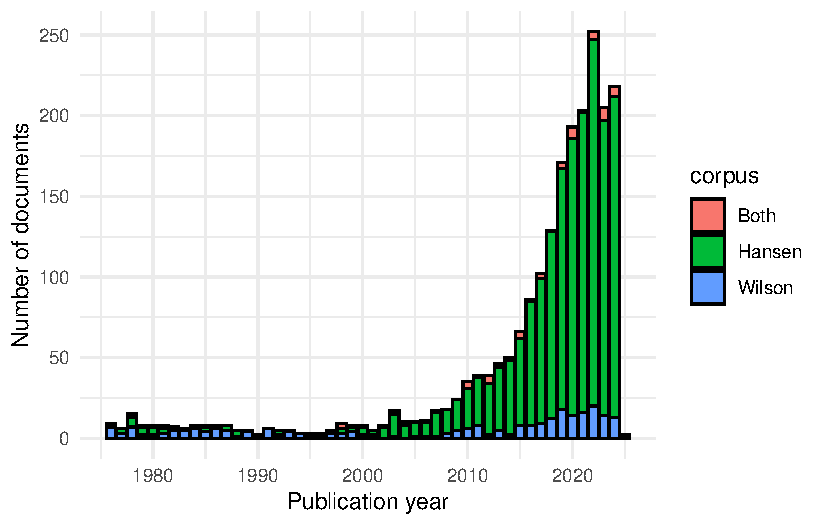
\includegraphics[width=0.7\textwidth,height=\textheight]{paper_plos_files/figure-pdf/fig-docs-per-year-1.pdf}

}

\caption{\label{fig-docs-per-year}Historical pattern of publication:
documents per year.}

\end{figure}%

Despite their close conceptual ties, the accessibility and spatial
interaction modeling literatures have developed along largely separate
paths since the 1970s. Hansen's \citep{hansen1959} formulation of
accessibility became the method used for decades of work on transport
equity, land use analysis, and urban accessibility planning. Meanwhile,
Wilson's \citep{wilson1971} entropy-maximising framework reshaped how
spatial interaction models were constructed, particularly in
transportation demand forecasting. We argue the framework's quiet
innovation--introducing empirically grounded constraints to shift from
proportionality to calibrated equality--made the framework immediately
relevant for policy applications as outputs were in tangible units. Yet,
this mechanism was never widely adopted in accessibility analysis.

This divergence is especially striking given the context in which both
frameworks emerged. As noted in
\citep{battyChronicleScientificPlanning1994}, large scale spatial
interaction models (like Wilson's) responded to important developments
at the time, a need ``to meet the dictates and needs of public policy
for strategic land use and transportation planning''. And these needs
were far from trivial: in the U.S., for instance, the Federal-Aid
Highway Act of 1956 set in motion the construction of the Interstate
Highway System with an eventual budget exceeding \$600 billion in
today's dollars
\citep{weinerUrbanTransportationPlanning2016, mdotMnDOTJoins2007}. In
this context, spatial interaction models were incorporated into
institutional practices focused on ``predict and provide'' travel demand
forecasting
\citep{kovatch1971modeling, weinerUrbanTransportationPlanning2016}.
Accessibility analysis, by contrast, remained more conceptually diffuse,
focused on indicators of ``potential'' spatial interaction with
opportunities rather than flows that could tangibly guide infrastructure
decisions (e.g., roadway capacity expansion, new construction). Whereas
spatial interaction modelling became a key element of transportation
planning practice, accessibility remained a somewhat more academic
pursuit, and the two streams of literature only rarely connected.

To explore why Wilson's approach never crossed over to accessibility
modeling, we conduct a review of the literature citing Hansen
\citep{hansen1959}, Wilson \citep{wilson1971}, or both (on Web of
Science using the ``Cited References'' functionality, and the digital
object identifiers of Hansen \citep{hansen1959} and Wilson
\citep{wilson1971}) . Only 76 out of the 2,122 documents that emerged
from our search cite both. The number of articles, by year and if they
cite Hasen, Wilson, or both are shown in Fig~\ref{fig-docs-per-year}.

Through the close analysis of \emph{how} articles that cite both works,
we identify two distinct citation patterns: one group of articles
focused on accessibility, the other on spatial interaction. In examining
these articles, we uncover how the relationship between the two has
often been misunderstood, underexplored, or entirely overlooked.

In the first stream of literature--which cite both but are focused more
so on spatial interaction models--they treat spatial interaction and
accessibility as separate but related phenomenons. Four subsets of this
stream emerge.

First, some of the more early works interpret the spatial interaction
model's balancing factors
(Eq~\ref{eq-production-constrained-balancing-factor} or
Eq~\ref{eq-doubly-constrained-balancing-factors}) as the inverse of
Hansen's accessibility measure
\citep{harrisEquilibriumValuesDynamics1978, leonardiOptimumFacilityLocation1978, fotheringhamSPATIALSTRUCTUREDISTANCE1981, fotheringhamSpatialCompetitionAgglomeration1985},
likely following Wilson's own recognition of this similarity between
balancing factor \(A_i\) and Hansen-type measure \(S_i\) on p.~10 in
Wilson \citep{wilson1971}. In some ways, this relationship has been
recognized as a ``common sense'' approach to incorporating accessibility
in the spatial interaction model
\citep[p.~99]{morrisAccessibilityIndicatorsTransport1979}, though
acknowledgment of its further exploration has been recommended
\citep{battyMethodResiduesUrban1976}.

The second subset of articles within this stream use both Hansen
\citep{hansen1959} and Wilson's \citep{wilson1971} framework in
conjunction. For instance, some articles argue that spatial interaction
models fail to explain certain spatial patterns on their own, for
instance, as in Fotheringham
\citep{fotheringhamSpatialCompetitionAgglomeration1985} who demonstrates
how the spatial interaction model may insufficiently explain spatial
patterns, and suggests that explicitly defining destinations'
accessibility (Hansen-type accessibility) as a variable within the model
may remedy the issue (e.g., the \emph{competition destination} model).
Other works take a more applied approach: such as in defining
location-allocation problems in operations research
\citep{leonardiOptimumFacilityLocation1978, beaumontLocationallocationProblemsPlane1981},
estimating trips (or some other spatial interaction flows) alongside
accessibility
\citep[e.g.,][]{clarke2002deriving, grengs2004measuring, turk2019socio},
or considering accessibility as a variable within spatial interaction
models, in line with Fotheringham's
\citep{fotheringhamSpatialCompetitionAgglomeration1985} demonstration
\citep[e.g.,][]{beckers2022incorporating}.

The third subset of the spatial-interaction focused literature, depart
from Hansen's \citep{hansen1959} definition, aligning instead with
microeconomic or utility-based interpretations of potential spatial
interaction e.g.,
\citep{morrisAccessibilityIndicatorsTransport1979, leonardiRandomUtilityDemand1984}.
In sum though, across these works, they recognize Hansen-type
accessibility as an indicator of `potential' but as a separate but
related concept to spatial interaction.

Moving onto the group of accessibility-focused literature that cites
both works, we categorise their citation of Wilson \citep{wilson1971}
within three general groups. Overall though, these works do not engage,
or only superficially engage with Wilson \citep{wilson1971}.

Firstly, there is a group of articles within this stream that cite
Wilson \citep{wilson1971} exclusively as attribution for using
context-dependent travel cost functions. This trend is common: for
instance it is done in
\citep{weibullNumericalMeasurementAccessibility1980, handyMeasuringAccessibilityExploration1997, kwan1998space, shenLocationCharacteristicsInnercity1998, ashiru2003space, rau2012spatial, pan2013impacts, margaridacondecomelhoradoImpactMeasuringInternal2016, caschili2015accessibility, grengs2015nonwork, pan2020measuring, chia2020extending, roblot2021participation, sharifiasl2023incorporating, kharel2024examining}.
However, these works do not engage with spatial interaction beyond this
attribution.

Secondly, a subset of literature explicitly associates spatial
interaction, as defined in Wilson \citep{wilson1971}, with
accessibility's potential for spatial interaction--but only
superficially. These works acknowledge the conceptual link, but do not
go beyond this recognition in the scope of their works e.g.,
\citep{millerMeasuringSpaceTimeAccessibility1999, giuliano2010accessibility, grengs2010intermetropolitan, grengs2010job, grengs2012equity, levine2012does, levinson2012positive, tong2015transportation, liu2015spatial, he2017measuring, wuUnifyingAccess2020, ng2022reflection, naqavi2023mobility, suel2024measuring}.
Indeed, while accessibility can be seen as the \emph{potential} for
spatial interaction--and Wilson \citep{wilson1971} briefly touches on
this--such mentions have not resulted in deeper analytical integration
of these concepts. Furthermore, some of this literature also
occasionally conflates or blurs the distinction entirely, for instance
by co-citing Hansen and Wilson as being `gravity models'
\citep[e.g.,][]{liu2004accessibility, dai2017visualization, shen2019segregation, chia2020extending}.
This conflation reveals ongoing murkiness between the distinction of
spatial interaction and the \emph{potential for} spatial interaction in
the literature.

Thirdly, there is a group of accessibility-focused works that interprets
the measure used in Hansen \citep{hansen1959} as the singly- or doubly-
constrained spatial interaction model's inverse balancing factor
\citep[e.g.,][]{vickermanAccessibilityAttractionPotential1974}. This
group often cites the spatial interaction works that make this
connection (i.e., the first subset of the first stream of literature)
and is especially prominent in the investigation of competitive
accessibility topics e.g.,
\citep{karstEvaluationAccessibilityImpacts2003, geurs2006accessibility, willigers2007accessibility, el2011place, curtis2010planning, manaugh2012makes, chen2013regional, alonso2014labour, albacete2017measuring, sahebgharani2019computing, mayaud2019future, allenMeasureCompetitiveAccess2020, levinsonGeneralTheoryAccess2020, marwal2022literature, su2023untangling}.
Only the works of Soukhov et al.
\citep{soukhovIntroducingSpatialAvailability2023, soukhovMultimodalSpatialAvailability2024}
use Wilson's \citep{wilson1971} balancing factors as a method for
maintaining constraints on opportunities within the context of
competitive accessibility.

On that note, Soukhov et al., 2023 and 2024
\citep{soukhovIntroducingSpatialAvailability2023, soukhovMultimodalSpatialAvailability2024}
introduce the balancing factors as a mechanisms to ensure that
opportunities at each destination are proportionally allocated to each
zone (based on the proportion of population seeking opportunities and
the relative travel impedance). This is to ensure that each zonal
accessibility value is the sum of this proportional allocation from each
destination, and that all zonal values ultimately sum to the total
number of opportunities in the region. However, these balancing factors
were deduced intuitively. These works do not explicitly state that the
mathematical formulation of the equations are effectively equivalent to
Wilson's singly constrained model (derived from entropy maximization).
This equivalence is only discovered in hindsight, as will be
demonstrated in the following section. These two works also do not
discuss other constrained cases that will also be addressed.

In sum, despite the interpretative advantaged offered by the statistical
logic of Wilson \citep{wilson1971}'s framework, the spatial
interaction-oriented Hansen \citep{hansen1959} citing literature nor the
accessibility-oriented literature that cite Wilson \citep{wilson1971}
have yet to meaningfully adopt Wilson's constraint-based logic to the
concept of accessibility. So, in the next section, we demonstrate how
applying Wilson's framework enables accessibility to move from a
proportional relationship to calibrated equality--tying outputs to
tangible system knowns. This re-expression of accessibility using
constraints yields interpretable, unit-consistent measures of
opportunity. This approach takes the same path of entropy-maximisation
as in Wilson \citep{wilson1971}, and does not rely on specifying some
universal constant \(G\) like initially proposed in Stewart
\citep{stewartDemographicGravitationEvidence1948} (recall,
Eq~\ref{eq-stewart-population-potential-sum} which Hansen
\citep{hansen1959} operationalised).

\section{A family of accessibility measures: from proportionality to
equality}\label{a-family-of-accessibility-measures-from-proportionality-to-equality}

Despite the close conceptual ties between accessibility and spatial
interaction modeling, the former has not meaningfully absorbed the
constraint-based logic of the latter. This section introduces this
reframing: defining a family of accessibility measures using Wilson's
approach grounded in statistical mechanics, shifting place-based
accessibility (a la Hansen \citep{hansen1959}) from a relationship
describing proportionality to equality.

This shift addresses the fundamental issue of interpretability
associated with the proportional nature of Hansen-type accessibility
indicators we previous outlined. Rather than relying on arbitrary or
uncalibrated proportional relationships (or invoking a universal
constant \(G\) as proposed in Stewart
\citep{stewartDemographicGravitationEvidence1948}) we adopt Wilson's
approach grounded in statistical mechanics.

To do so, we propose a revised definition of accessibility considerate
of the constraint-based spatial interaction model: the potential for
spatial interaction with opportunities (or population). We can specify
\(k\) as a type of proportional allocation factor \(\kappa\) which
incorporates Wilson's balancing factor(s) to define the \emph{potential
for spatial interaction with opportunities} \(V_{ij}\) and the
\emph{potential for spatial interaction with population} \(M_{ji}\). In
effect, \(\kappa\) is unitless and proportionally allocates (based on
the constraints of the case) opportunities (for \(V_{ij}\)) and
population (for \(M_{ji}\)). The equation is as follows:

\begin{equation}\phantomsection\label{eq-access-01}{
\begin{array}{l}
V_{ij}^X = \kappa_{ij}^X W_X^{(2)}\\ 
M_{ji}^X = \hat \kappa_{ji}^X W_X^{(1)}
\end{array}
}\end{equation}

\noindent Where \(W_X^{(2)}\) and \(W_X^{(1)}\) is the mass of the
destination (i.e., opportunities) and mass of the origin (i.e.,
population) at either the zone or for the full region, depending on the
case (hence represented by a \(X\)).

Accessibility flows can also be summarised as as a partial sum of the
potential at \(i\) and at \(j\) to express accessibility at the origin
zone or at the destination zone, respectively, as often done in
accessibility research:

\begin{equation}\phantomsection\label{eq-accesssibility-01}{
\begin{array}{l}
V_{i}^X = \sum_j \kappa_{ij}^X W_X^{(2)}\\
M_{j}^X = \sum_i \hat \kappa_{ji}^X W_X^{(1)}
\end{array}
}\end{equation}

Figure Fig~\ref{fig-analytical-device-conc-accessibility} illustrates
our analytical framework using a simple 3-zone system. The most detailed
values, \(X_{ij}\), represent the potential for spatial interaction from
origin \(i\) to destination \(j\). Here, \(X\) stands for all cases and
variants to be discussed (e.g., \(V_{ij}^0\), \(M_{ji}^0\),
\(V_{ij}^T\), \(M_{ji}^T\), \(V_{ij}^S\), \(M_{ji}^S\), \(V_{ij}^D\),
and \(M_{ji}^D\)). Single marginals show origin and destination weights,
while the total marginal sums these values.

\begin{figure}[H]

\centering{

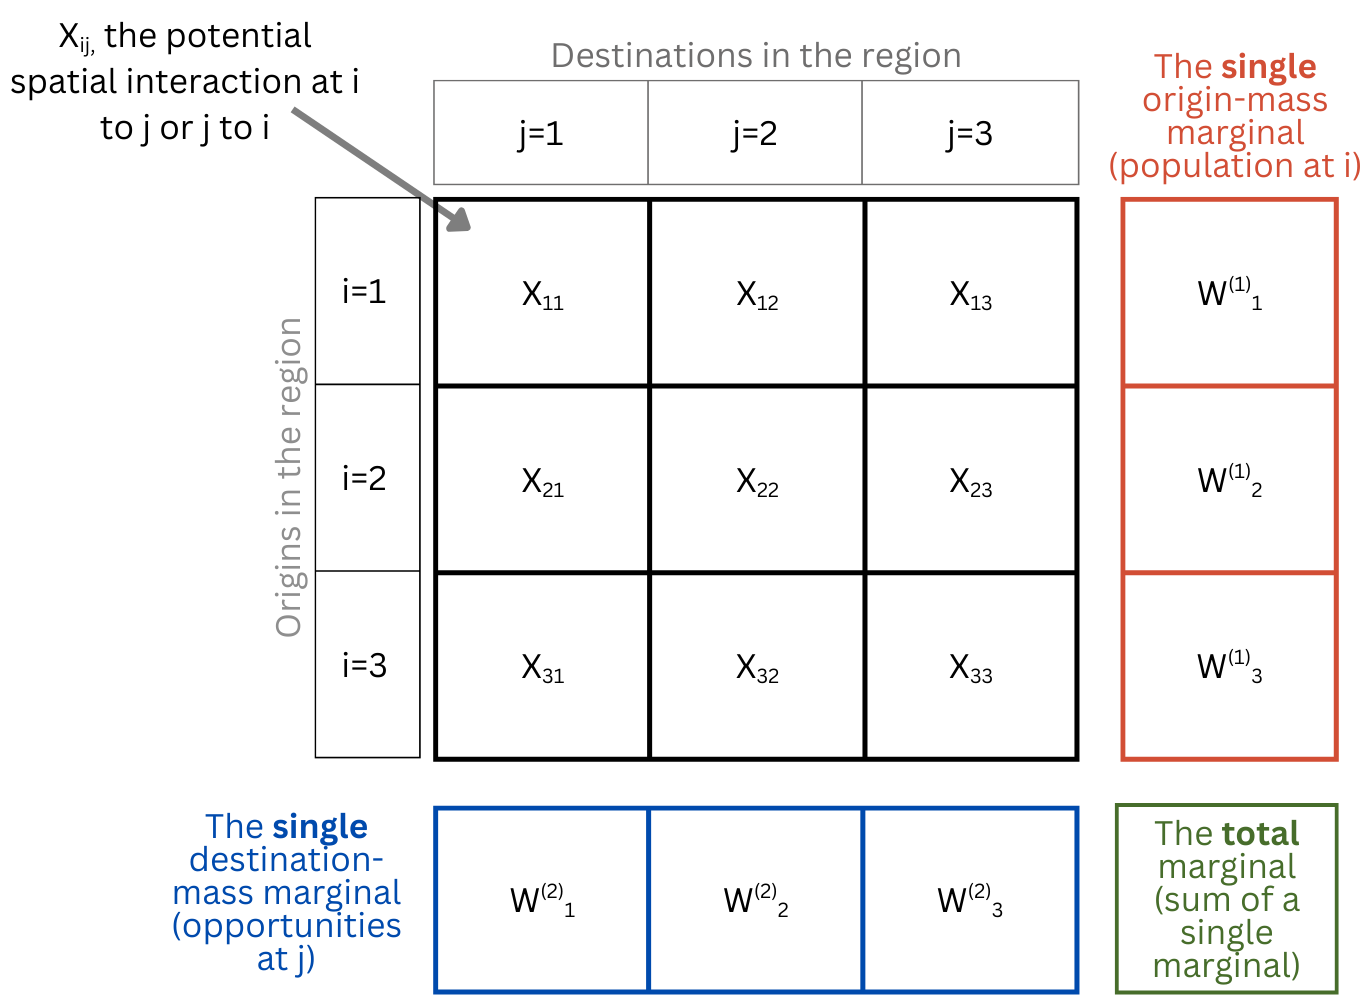
\includegraphics[width=0.7\textwidth,height=\textheight]{../figures/access-analytical-device.png}

}

\caption{\label{fig-analytical-device-conc-accessibility}The family of
accessibility measures analytical framework: labelling and associating
ij flows, zonal weights, the single marginals, and the total marginal.}

\end{figure}%

The proportional allocation constant \(\kappa\) takes the form of a
balancing factor that varies depending on the constraints applied. Each
member of the accessibility measure family is defined by the constraints
used, and can be grouped into the following four cases:

\begin{enumerate}
\def\labelenumi{\arabic{enumi}.}
\tightlist
\item
  \textbf{Unconstrained Case (\(V_i^0\), \(M_j^0\))}
\end{enumerate}

\begin{itemize}
\tightlist
\item
  Equivalent to Hansen's \citep{hansen1959} and Reilly's
  \citep{reilly1929methods} original formulations; the status quo of
  accessibility modelling.
\item
  No balancing factors applied; units are in
  ``opportunities-by-impedance'' for \(V_i^0\) or
  ``population-by-impedance'' for \(M_j^0\).
\item
  No constraints are applied, so values reflect proportionality only and
  are not calibrated to known system totals.
\end{itemize}

\begin{enumerate}
\def\labelenumi{\arabic{enumi}.}
\setcounter{enumi}{1}
\tightlist
\item
  \textbf{Total Constrained Case (\(V_i^T\), \(M_j^T\))}
\end{enumerate}

\begin{itemize}
\tightlist
\item
  Applies a total proportional allocation factor (\(\kappa_{ij}^T\),
  \(\hat \kappa_{ji}^T\)) based only on the total marginal (green box in
  Fig~\ref{fig-analytical-device-conc-accessibility}) i.e., total number
  of opportunities or population in the system. This ensures the sum of
  all values in the system match the total marginal.
\item
  Units of \(V_i^T\): accessible opportunities from \(i\), a value that
  is total constrained and linearly proportion to \(V_i^0\).
\item
  Units of \(M_j^T\): accessible population from \(j\), a value that is
  total constrained and linearly proportion to \(M_j^0\).
\end{itemize}

\begin{enumerate}
\def\labelenumi{\arabic{enumi}.}
\setcounter{enumi}{2}
\tightlist
\item
  \textbf{Singly Constrained Case (\(V_i^S\), \(M_j^S\))}
\end{enumerate}

\begin{itemize}
\tightlist
\item
  Applies singly-constrained proportional allocation factors
  (\(\kappa_{ij}^S\), \(\hat \kappa_{ji}^S\)) based on Wilson's
  balancing factors (\(B_j\), \(A_i\)) to preserve either the
  destination-side or origin-side marginal totals (blue and red boxes in
  Fig~\ref{fig-analytical-device-conc-accessibility}) i.e., the number
  of opportunities or population at each zone. Reflects how the
  literature calculates competitive accessibility.
\item
  Units of \(V_i^S\): accessible opportunities from \(i\), a value that
  is the sum of opportunity supply flows allocated proportionally based
  on demand at \(i\). Mathematically equivalent in per-capita form to
  2SFCA \citep{luo2003}.
\item
  Units of \(M_j^S\): accessible population from \(j\), a value that is
  the sum of population demand flows allocated proportionally based on
  supply at \(j\).
\end{itemize}

\begin{enumerate}
\def\labelenumi{\arabic{enumi}.}
\setcounter{enumi}{3}
\tightlist
\item
  \textbf{Doubly Constrained Case (\(V_{ij}^D\), \(M_{ji}^D\))}
\end{enumerate}

\begin{itemize}
\tightlist
\item
  Constrained on both origin and destination sides using both \(A_i\)
  and \(B_j\) simultaneously, which can also be expressed as
  proportional allocation factors (\(\kappa_{ij}^D\),
  \(\hat \kappa_{ji}^D\)); equivalent in interpretation to Wilson's
  \citep{wilson1971} doubly constrained spatial interaction model.
\item
  Simultaneous application ensures both the destination-side \emph{and}
  origin-side marginal totals are maintained (blue and red boxes in
  Fig~\ref{fig-analytical-device-conc-accessibility}).
\item
  Interpretable only as \(ij\) and \(ji\) flows, since aggregation at
  \(i\) and \(j\) simply reproduces known totals. Represents
  `interaction capacity' or `realized access' serving as predictions of
  real interaction flows.
\end{itemize}

\subsection{Toy example setup}\label{toy-example-setup}

Consider the simple 3-zone region in Figure
Fig~\ref{fig-analytical-device-conc-accessibility}, where each zone
serves as both origin (\(i\)) and destination (\(j\)). The system
includes three inputs: zonal population and opportunities, a zonal cost
(travel time) matrix, and three travel impedance functions representing
different travel behaviours.

First, Table Table~\ref{tbl-small-system-land-use} summarizes population
(in 10,000s) and physicians per zone. For context, the
Provider-to-Population Ratio (PPR) is 24.5 comparable to Canada's 2022
PPR of 24.97 physicians per 10,000 \citep{whoMedicalDoctors102025}.
Second, Table Table~\ref{tbl-small-system-cost} shows travel times
(minutes); it can be discerned that Zones 1 and 3 are closer to each
other than to Zone 2. Zones 1 and 3 together have a population roughly
equal to Zone 2 but offer more than twice the physician availability. We
interpret Zone 1 as the Urban Edge, Zone 3 as part of the Urban Core,
and Zone 2 as the Suburban.

\begin{table}

\caption{\label{tbl-small-system-land-use}Simple system with three zones
(ID 1, 2 and 3). Population is in 10,000 persons and opportunities in
number of physicians.}

\centering{

\fontsize{7.5pt}{9.0pt}\selectfont
\begin{tabular*}{\linewidth}{@{\extracolsep{\fill}}rcc}
\toprule
ID (i or j) & Population\textsuperscript{\textit{1}} & Opportunities\textsuperscript{\textit{2}} \\ 
\midrule\addlinespace[2.5pt]
1 & 4 & 160 \\ 
2 & 10 & 150 \\ 
3 & 6 & 180 \\ 
\bottomrule
\end{tabular*}
\begin{minipage}{\linewidth}
\textsuperscript{\textit{1}}Population is \emph{Wi\textsuperscript{(1)}} when used as a proxy for the mass at the origin, and \emph{Oi} when used as a constraint.\\
\textsuperscript{\textit{2}}Opportunities is \emph{Wj\textsuperscript{(2)}} when used as a proxy for the mass at the destination, and \emph{Dj} when used as a constraint.\\
\end{minipage}

}

\end{table}%

\begin{table}

\caption{\label{tbl-small-system-cost}Cost matrix for system with three
zones (travel time in minutes).}

\centering{

\fontsize{7.5pt}{9.0pt}\selectfont
\begin{tabular*}{\linewidth}{@{\extracolsep{\fill}}cccc}
\toprule
 & \multicolumn{3}{c}{Destination ID} \\ 
\cmidrule(lr){2-4}
Origin ID & 1 & 2 & 3 \\ 
\midrule\addlinespace[2.5pt]
1 & 10 & 30 & 15 \\ 
2 & 30 & 10 & 25 \\ 
3 & 15 & 25 & 10 \\ 
\bottomrule
\end{tabular*}

}

\end{table}%

And third, Eq~\ref{eq-travel-behaviour-scenarios} presents the assumed
travel impedance functions reflecting three different travel behaviours.
A helpful analogy may be tying travel behaviour to the used mode's
mobility potential, i.e., the most decaying travel behaviour
(\(f_1(c_{ij})\)) would assume all travel in the region being done by
foot, while calculating accessibility assuming the least decay
(\(f_3(c_{ij})\)) would assume unfettered automobility.

\begin{equation}\phantomsection\label{eq-travel-behaviour-scenarios}{
\begin{array}{l}
f_1(c_{ij}) = \frac{1}{c_{ij}^3}\\
f_2(c_{ij}) = \frac{1}{c_{ij}^2}\\
f_3(c_{ij}) = \frac{1}{c_{ij}^{0.1}}
\end{array}
}\end{equation}

Any set of concepts representing population, opportunities, and their
associated travel behaviour, whether representing the entire region
uniformly (as will be demonstrated) or representing specific subgroups,
can be substituted into our simple toy example. The purpose of the
following simple example is to demonstrate the calculation and
interpretation of the four accessibility measure variants.

\subsection{Unconstrained
accessibility}\label{unconstrained-accessibility}

In \(V^0_i\), no proportional allocation factor is defined, simply
\(f(c_{ij})\) is used to weight the number of opportunities at each
\(j\) and the weighted values for each \(j\) are summed for each \(i\),
yielding the an expression identical to Hansen's accessibility \(S_i\)
\citep{hansen1959}, the current standard practice in accessibility
measurement:

\begin{equation}\phantomsection\label{eq-unconstrained-accessibility}{
V^0_i = \sum_j V^0_{ij} = \sum_j W^{(2)}_jf(c_{ij}) = S_i
}\end{equation}

However \(\sum_i V^0_{i}\) generally does not equal the total
opportunities \(O\), so units here are `opportunities weighted by travel
impedance' and lack meaningful scaling or direct interpretability.
Comparing values across different decay functions or contexts (i.e.,
different number of zones) is therefore limited to ordinal statements
(more vs.~less), not intervals or ratios (i.e., the magnitude of
differences).

\begin{table}

\caption{\label{tbl-simple-example-unconstrained-accessibility}Simple
system: unconstrained accessibility.}

\centering{

\fontsize{6.0pt}{7.2pt}\selectfont
\begin{tabular*}{\linewidth}{@{\extracolsep{\fill}}l|ccc}
\toprule
 & \multicolumn{3}{c}{V\textsubscript{i}\textsuperscript{0}} \\ 
\cmidrule(lr){2-4}
 & f\textsubscript{1} (c\textsubscript{ij}) = 1/c\textsubscript{ij}\textsuperscript{3} & f\textsubscript{2} (c\textsubscript{ij}) = 1/c\textsubscript{ij}\textsuperscript{2} & f\textsubscript{3} (c\textsubscript{ij}) = 1/c\textsubscript{ij}\textsuperscript{0.1} \\ 
\cmidrule(lr){2-2} \cmidrule(lr){3-3} \cmidrule(lr){4-4}
Origin & units: \emph{physicians-minute\^{}-3} & units: \emph{physicians-minute\^{}-2} & units: \emph{physicians-minute\^{}-0.1} \\ 
\midrule\addlinespace[2.5pt]
1 & 0.219 & 2.567 & 371.143 \\ 
2 & 0.167 & 1.966 & 363.479 \\ 
3 & 0.237 & 2.751 & 373.738 \\ 
\midrule 
\midrule 
Sum & 0.6233422 & 7.283556 & 1108.361 \\ 
\bottomrule
\end{tabular*}

}

\end{table}%

For example, Table
Table~\ref{tbl-simple-example-unconstrained-accessibility} shows
\(V^0_{i}\) under each decay function. Comparing across decay types is
meaningless in absolute terms. For instance, the difference in zone 1
(edge of urban core)'s accessibility under \(f_3\) vs \(f_1\) is 370.92,
but in what units? These two values are a product of different impedance
functions ( \emph{physicians-minute\(^{-3}\)} and
\emph{physicians-minute\(^{-0.1}\)}), making the comparison
uninterpretable (and arguably incorrect). The fundamental
uninterpretability of what is a
\emph{opportunity-weighted-travel-impedance} unit remains.

As the different impedance functions represent different travel
behaviours, comparing the raw unconstrained accessibility values across
groups is meaningless beyond notions of higher or lower. While one could
attempt to adjust the units post-calculation (e.g., scaling, population
normalization) or select impedance functions to facilitate comparison
across scenarios (potentially at the expense of accurately reflecting
travel behavior), such adjustments may introduce bias. The unconstrained
scores are best used for ranking within a single context.

The next sections introduce constraints to calibrate these measures for
better interpretability and comparability, applying each to this example
in turn.

\subsection{Total constrained
accessibility}\label{total-constrained-accessibility}

The total constrained accessibility case can be interpreted in a few
ways. In the one that connects to the status quo: the total balancing
factor proportionally adjusts unconstrained zonal accessibility values
\(V^0_i\) so their total sum of \(V^0_i\) matches a known system
total--either total opportunities or total population. Another
interpretation is in reformulating the equation to use a a proportional
allocation constant based on the total balancing factor. The
proportional allocation constant distributes opportunities (or
population) proportionally by travel impedance.

In both formulations, all zonal values become a proportion of a known
system total, be it the regional opportunities or regional population
depending on the variant.

We define two variants for this case:

\begin{itemize}
\tightlist
\item
  \(V_i^T\): accessibility is constrained by the total number of
  opportunities (total constrained accessible opportunity) and which is
  interpreted as Hansen's accessibility with a constraining constant,
  and
\item
  \(M_j^T\): where \(i\) and \(j\) of the first variant is transposed,
  yielding a measure constrained by the total number of population and
  to be interpreted as constrained `market potential'.
\end{itemize}

\subsubsection{Total constrained accessible opportunities: Hansen's
accessibility with a total
constraint}\label{total-constrained-accessible-opportunities-hansens-accessibility-with-a-total-constraint}

In the total constrained case, accessibility is expressed as a share of
the total number of opportunities in the region \(D\), allocated based
on travel impedance. The total constrained accessibility from \(i\) to
\(j\):
\begin{equation}\phantomsection\label{eq-total-constrained-access}{
V^T_{ij} = \kappa_{ij}^T D
}\end{equation}

This formulation satisfies the total constraint, analogous to the one in
the Wilson framework:
\begin{equation}\phantomsection\label{eq-total-constraint-D}{
\sum_i \sum_j V^T_{ij} =  D
}\end{equation}

Next, the proportional allocation factor \(\kappa_{ij}^T\) determines
the share of total opportunities assigned to each origin--destination
pair, based on the relative proportion of opportunities-weighted travel
impedance: \[
\kappa_{ij}^T = \frac{W^{(2)}_j f(c_{ij})}{\sum_i\sum_j W^{(2)}_jf(c_{ij})}
\] This renders \(V_i^T\) (equal to \(\sum_jV_{ij}^T\)) into units of
opportunities (e.g., physicians), and allows direct interpretation and
comparison of results between zones and scenarios.

Alternatively, this formulation can be rewritten to be expressed using a
total constrained balancing factor \(K^T\), which scales Hansen's
unconstrained accessibility \(V_i^0\) to meet the total opportunity
constraint:
\begin{equation}\phantomsection\label{eq-total-constrained-accessibility}{
V^T_i = \sum_j V^T_{ij} = K^T \sum_j W^{(2)}_jf(c_{ij}) = K^T  V^0_i
}\end{equation}

Where the total constrained balancing factor \(K^T\) is:
\begin{equation}\phantomsection\label{eq-total-opportunity-balancing-factor}{
K^T = \frac{D}{\sum_i\sum_j W^{(2)}_jf(c_{ij})}
}\end{equation}

This expression is consistent with Wilson's entropy-maximizing framework
and analogous to the total flow spatial interaction model (e.g.,
Equation 2.11 in \citep{cliff_evaluating_1974}).

In summary, \(\kappa_{ij}^T\) proportionally allocates the total number
of opportunities \(D\) to each origin--destination pair based on
relative opportunity-weighted travel impedance. These values can be
aggregated across destinations to obtain total constrained accessibility
at each origin. Alternatively, the measure can be expressed using the
balancing factor \(K^T\), demonstrating that it is algebraically
proportional to unconstrained accessibility \(V_i^0\), but with
interpretable units (i.e., opportunities). This allows for meaningful
comparisons of differences across zones and travel behaviour scenarios.

Referring back to our simple numeric example, \(K^T\) for the highest
decay t scenario \(f_1(c_{ij}) = 1/c_{ij}^3\) would then be:

\[
K^T = \frac{D}{\sum_{i}\sum_{j} W_j^{(2)} f(c_{ij})} = \frac{490}{0.6233} = 786.085
\]

\(K^T\) for other decay scenarios are calculated similarly in code.
Applying each \(K^T\) to the unconstrained values \(V_i^0\) yields total
constrained accessibility values (Table
Table~\ref{tbl-simple-example-total-opportunity-accessibility}), all in
units of physicians.

\begin{table}

\caption{\label{tbl-simple-example-total-opportunity-accessibility}Simple
system: total constrained accessible opportunities.}

\centering{

\fontsize{6.0pt}{7.2pt}\selectfont
\begin{tabular*}{\linewidth}{@{\extracolsep{\fill}}l|ccc}
\toprule
 & \multicolumn{3}{c}{V\textsubscript{i}\textsuperscript{T}} \\ 
\cmidrule(lr){2-4}
 & f\textsubscript{1} (c\textsubscript{ij}) = 1/c\textsubscript{ij}\textsuperscript{3} & f\textsubscript{2} (c\textsubscript{ij}) = 1/c\textsubscript{ij}\textsuperscript{2} & f\textsubscript{3} (c\textsubscript{ij}) = 1/c\textsubscript{ij}\textsuperscript{0.1} \\ 
\cmidrule(lr){2-2} \cmidrule(lr){3-3} \cmidrule(lr){4-4}
Origin & units: \emph{physicians} & units: \emph{physicians} & units: \emph{physicians} \\ 
\midrule\addlinespace[2.5pt]
1 & 172.065 & 172.672 & 164.080 \\ 
2 & 131.627 & 132.247 & 160.692 \\ 
3 & 186.308 & 185.081 & 165.228 \\ 
\midrule 
\midrule 
Sum & 490 & 490 & 490 \\ 
\bottomrule
\end{tabular*}

}

\end{table}%

Compared to the unconstrained case, values now sum to the known regional
total \(D\), allowing interpretation of absolute and relative
differences across zones and travel scenarios. For example, in the
highest decay case, Zone 1 (Urban Edge) captures an intermediate number
of physicians (172.0652825), like in the unconstrained accessibility
case. However, unlike in the unconstrained case, we can say that this
value is out of the 490 physicians in the region, which allows us also
to deduce that zone 1 captures 1.3072213 and 0.9235529 times more than
zone 2 and 3. Values for the lesser decay (\(f_2(c_{ij})\)) and lowest
decay (\(f_3(c_{ij})\)) scenarios are calculated separately, with decay
scenario values also summing to equal 490 physicians accessible in the
region.

One can also directly compare values at a specific zone, across travel
impedance scenarios, due to the consistent units. As the decay scenario
decreases, all zones become more accessible to each other and the
differences between pairs diminishes (i.e., in \(f_3(c_{ij})\) each zone
captures close to an average amount of physicians, a third of 490 or
\textasciitilde163). This averaging of the total amount is how the total
constrained proportional allocation factor functions. However, what's
notable is how Zones change between scenarios. For instance, Zone 1's
share only declines slightly--these declines are outpaced by Zone 2's
relative gains. This shift reflects how \(\kappa_{ij}^T\) redistributes
opportunities in proportion to impedance under different travel
behaviours.

The total constrained accessibility measure resolves the
interpretability issue of Hansen's accessibility (i.e., unconstrained
accessibility) by grounding values in a meaningful total, enabling
robust comparisons across zones and scenarios but also by keeping values
proportional to \(V_i^0\) so interpretation is similar.

\subsubsection{Total constrained accessible population: Reilly's
potential trade territories with a total
constraint}\label{total-constrained-accessible-population-reillys-potential-trade-territories-with-a-total-constraint}

This second total constrained variant is a transpose of the
opportunity-constrained formulation, switching indices \(i\) and \(j\)
to yield s measure of market potential--the number of people who can
spatially interact with a destination.

Though not outlined in the ``Unconstrained accessibility'' section, the
unconstrained form aligns with Reilly's ``potential trade territories''
\citep{reilly1929methods} and Harris' and Vickerman's formulations of
regional market potential
\citep{harris_market_1954, vickermanAccessibilityAttractionPotential1974}.
In its unconstrained form, market potential has also been more recently
to estimate potentially accessible populations following infrastructure
investments
\citep[e.g.,][]{gutierrezLocationEconomicPotential2001, holl2007twenty, condecco2018road}.
Market potential can also be thought of as a form of \emph{passive
accessibility}, indicating the number of people that can reach each
destination.

However, like \(V_{ij}^0\), issues of unit interpretability arise in
unconstrained market potential \(M_j^0\). To address this, we introduce
the total constrained accessible population measure \(M^T_{ji}\), which
allocates the total population \(O\) across all origin-destination pairs
proportionally:

\begin{equation}\phantomsection\label{eq-total-constrained-market}{
M^T_{ji} = \kappa_{ji}^T O
}\end{equation}

\noindent Subject to the total constraint::
\begin{equation}\phantomsection\label{eq-total-constraint-O}{
\sum_i \sum_j M^T_{ji} =  O
}\end{equation}

Next, \(\hat \kappa_{ij}\) is the total constrained proportional
allocation factor, a dimensionless term which distributes population
based on impedance-weighted accessibility: \[
\hat \kappa_{ij}^T = \frac{W^{(1)}_i f(c_{ij})}{\sum_i\sum_j W^{(1)}_if(c_{ij})}
\]

This renders \(M_j^T\) (equal to \(\sum_jM_{ji}^T\)) into units of
population. Alternatively, this formulation can be rewritten to be
expressed using a total constrained balancing factor \(\hat K^T\), which
scales unconstrained market potential \(M_j^0\) to meet the total
population constraint:
\begin{equation}\phantomsection\label{eq-total-constrained-market-potential}{
M^T_j = \sum_i M^T_{ji} = \hat K^T \sum_i W^{(1)}_if(c_{ij}) = \hat K^T  M^0_j
}\end{equation}

Where the total constrained balancing factor \(\hat K^T\) is:
\begin{equation}\phantomsection\label{eq-total-population-balancing-factor}{
\hat K^T = \frac{D}{\sum_i\sum_j W^{(1)}_if(c_{ij})}
}\end{equation}

In summary, \(\hat \kappa_{ij}^T\) allocates the total number of
population \(O\) proportionally to each origin--destination pair based
on relative population-weighted travel impedance. As well, the measure
can be expressed using the balancing factor \(\hat K^T\), demonstrating
that it is algebraically proportional to unconstrained market potential,
but also yielding interpretable units that allow for meaningful
comparison.

Returning to the numerical example, the balancing factor \(\hat K^T\) is
solved for each travel behaviour scenario, and the market potential of
each zone \(M^T_j\) is expressed as units of population (e.g., the
number of people accessible from each origin at that destination) in
Table~\ref{tbl-simple-example-total-population-accessibility}.

\begin{table}

\caption{\label{tbl-simple-example-total-population-accessibility}Simple
system: total constrained accessible population.}

\centering{

\fontsize{6.0pt}{7.2pt}\selectfont
\begin{tabular*}{\linewidth}{@{\extracolsep{\fill}}l|ccc}
\toprule
 & \multicolumn{3}{c}{M\textsubscript{i}\textsuperscript{S}} \\ 
\cmidrule(lr){2-4}
 & f\textsubscript{1} (c\textsubscript{ij}) = 1/c\textsubscript{ij}\textsuperscript{3} & f\textsubscript{2} (c\textsubscript{ij}) = 1/c\textsubscript{ij}\textsuperscript{2} & f\textsubscript{3} (c\textsubscript{ij}) = 1/c\textsubscript{ij}\textsuperscript{0.1} \\ 
\cmidrule(lr){2-2} \cmidrule(lr){3-3} \cmidrule(lr){4-4}
Destination & units: \emph{population in 10,000s} & units: \emph{population in 10,000s} & units: \emph{population in 10,000s} \\ 
\midrule\addlinespace[2.5pt]
1 & 5.018 & 5.447 & 6.598 \\ 
2 & 8.596 & 7.986 & 6.717 \\ 
3 & 6.386 & 6.567 & 6.684 \\ 
\midrule 
\midrule 
Sum & 20 & 20 & 20 \\ 
\bottomrule
\end{tabular*}

}

\end{table}%

Readers may note the difference in trends in accessible population
(Table~\ref{tbl-simple-example-total-population-accessibility}) and
accessible physicians (i.e., the preceding subsection,
Table~\ref{tbl-simple-example-total-opportunity-accessibility}).

In Table~\ref{tbl-simple-example-total-opportunity-accessibility}, zone
1, 2, 3 represent destinations and the accessibility values reflect the
number of accessible people from the vantage of physicians. Zone 1, in
its role as a destination, is no longer intermediately-ranked relative
to other zones; it now attracts the fewest number of people across all
three travel behaviour scenarios. However, similar to the total
constrained opportunity case, as travel decay reduces, the availability
of population begins to converge (though Zone 1 continues as the
lowest-ranked) for similar reasons. As decay reduces, the population's
travel impedance to all zones become more similar, making the relative
location of the zones less important and all people in the region more
equally accessible.

Like in the total constrained accessible opportunities variant, the
total constrained accessible population enables direct comparison of raw
values, supporting both ordinal and interval interpretations across
space and travel behaviour scenarios.

\subsection{Singly constrained
accessibility}\label{singly-constrained-accessibility}

The singly constrained accessibility case can also be expressed in two
variants, each defined by the direction in which a constraint is
applied:

\begin{itemize}
\tightlist
\item
  \(V_i^S\): accessibility constrained by opportunities at destinations
  (singly constrained accessible opportunities), and
\item
  \(M_j^S\): its transpose, constrained by population at origins (singly
  constrained accessible population, or market potential).
\end{itemize}

Similar to the total constrained case, the singly constrained measures
adjust unconstrained zonal accessibility values (\(V_i^0\) or \(M_j^0\))
using a balancing factor to satisfy the known system constraint.
However, unlike the total constraint (which enforces a global/total
sum), the singly constrained case applies a localized constraint at one
end of the interaction--either origin or destination.

In the opportunities-constrained variant, the balancing factor ensures
that only a proportion of opportunities at each destination are
allocated to origins, based on their relative demand (population) and
travel impedance. This variant mirrors the concept of spatial
availability as discussed in Soukhov et al.
\citep{soukhovIntroducingSpatialAvailability2023}. In the
population-constrained variant, the logic is reversed: population at
each origin is allocated proportionally across destinations, informed by
the distribution of opportunities and impedance.

In both cases, the singly constrained formulation introduces zonal-level
competition, unlike the total constrained case which distributes a fixed
regional sum. Each zonal accessibility value becomes not only a fraction
of the regional total (opportunities or population), but also a balanced
sum of interactions, weighted by impedance and relative competition. The
result remains in interpretable units--accessible opportunities or
accessible population--but reflects more complex spatial dynamics.

\subsubsection{Singly constrained accessible opportunities: spatial
availability}\label{singly-constrained-accessible-opportunities-spatial-availability}

In this singly constrained variant, accessibility is constrained at the
destination side: the sum of accessible opportunities allocated from
each destination must equal the known number of opportunities \(D_j\).
This is comparable to the single attraction-constraint
(Eq~\ref{eq-constraint2-gravitymodel}) from Wilson's framework:

\begin{equation}\phantomsection\label{eq-opportunity-constraint}{
\sum_i V^S_{ij} =  D_j
}\end{equation}

The underlying spatial interaction model is now the
attraction-constrained model and our accessibility measure becomes:

\begin{equation}\phantomsection\label{eq-opportunity-constrained-accessibility}{
V^S_{i} = \sum_j B_j D_j W_i^{(1)} f(c_{ij})
}\end{equation}

\noindent where \(W_i^{(1)}\) is a measure of the mass at origin \(i\)
(i.e., the opportunity-seeking population). The corresponding balancing
factor, as per Wilson, is:

\begin{equation}\phantomsection\label{eq-opportunity-constrained-proportionality-constants}{
B_j = \frac{1}{\sum_i W_i^{(1)} f(c_{ij})}
}\end{equation}

Introducing the balancing factor in
Eq~\ref{eq-opportunity-constrained-accessibility}, we obtain:

\begin{equation}\phantomsection\label{eq-opportunity-constrained-accessibility-with-balancing-factor}{
V^S_{i} = \sum_j D_j \frac{W_i^{(1)} f(c_{ij})}{\sum_i W_i^{(1)} f(c_{ij})}
}\end{equation}

Further, we can express the formula even more simply, by defining the
following proportional allocation factor:

\begin{equation}\phantomsection\label{eq-opportunity-constrained-proportional-allocation-factor}{
\kappa^S_{ij} = \frac{W_i^{(1)} f(c_{ij})}{\sum_i W_i^{(1)} f(c_{ij})}
}\end{equation}

After this, it is possible to rewrite
Eq~\ref{eq-opportunity-constrained-accessibility-with-balancing-factor}
as an origin summary expression of proportionally allocated known
opportunities (i.e., \(D_j\)).

\begin{equation}\phantomsection\label{eq-attraction-constrained-accessibility-with-proportional-allocation-factor}{
V^S_{i} = \sum_j \kappa^S_{ij} D_j
}\end{equation}

This formulation has been referred to as \textbf{spatial availability}
by Soukhov et al. \citep{soukhovIntroducingSpatialAvailability2023},
since it incorporates spatial competition by allocating opportunities
based on demand (population), impedance, and the known opportunity
totals \(D_j\). The dimensionless factor \(\kappa^S_{ij}\) ensures that
each destination's opportunities are distributed proportionally to
origins. As in the total constrained case, \(V_i^S\) is expressed in the
units of accessible opportunities. Finally, the \textbf{per capita}
version of this measure:

Soukhov et al., 2023 \citep{soukhovIntroducingSpatialAvailability2023}
also showed that the following expression (accessibility per capita) is
a constrained version of the popular 2SFCA approach of Shen 1998
\citep{shen1998} and Luo and Wang 2003 \citep{luo2003}:

\begin{equation}\phantomsection\label{eq-opportunity-constrained-accessibility-per-capita}{
v^S_{i} = \frac{V^S_{i}}{W^{(1)}_i}
}\end{equation}

Returning to the simple numeric example, as an example of the solved
\(B_{j}\) for the highest decay travel behaviour \(f_1(c_{ij})\):

\[
\begin{array}{l}
B_{j} = \frac{1}{\sum_i W_i^{(1)} f(c_{ij})}\\
B_{1} =  \frac{1}{\frac{4}{10^3} + \frac{10}{30^3} + \frac{6}{15^3}} = 162.6506\\ 
B_{2} =  \frac{1}{\frac{4}{30^3} + \frac{10}{10^3} + \frac{6}{25^3}} = 94.9474\\
B_{3} =  \frac{1}{\frac{4}{10^3} + \frac{10}{25^3} + \frac{6}{10^3}} = 93.9850
\end{array}
\]

The balancing factors \(B_j\) for the \(f_2(c_{ij})\) decay group for
zones 1, 2 and 3 area 12.8571429, 8.7685113 and 10.6635071,
respectively. For the \(f_3(c_{ij})\) decay group, they are 0.0672461,
0.0660559 and 0.0663798. Using these these balancing constants, we can
calculate the singly constrained opportunity accessibility
(Table~\ref{tbl-simple-example-attraction-constrained-accessibility}).

\begin{table}

\caption{\label{tbl-simple-example-attraction-constrained-accessibility}Simple
system: singly constrained accessible opportunities.}

\centering{

\fontsize{6.0pt}{7.2pt}\selectfont
\begin{tabular*}{\linewidth}{@{\extracolsep{\fill}}l|cccc}
\toprule
 &  & \multicolumn{3}{c}{V\textsubscript{i}\textsuperscript{S}} \\ 
\cmidrule(lr){3-5}
 &  & f\textsubscript{1} (c\textsubscript{ij}) = 1/c\textsubscript{ij}\textsuperscript{3} & f\textsubscript{2} (c\textsubscript{ij}) = 1/c\textsubscript{ij}\textsuperscript{2} & f\textsubscript{3} (c\textsubscript{ij}) = 1/c\textsubscript{ij}\textsuperscript{0.1} \\ 
\cmidrule(lr){3-3} \cmidrule(lr){4-4} \cmidrule(lr){5-5}
Origin & Population (10k) & units: \emph{physicians} & units: \emph{physicians} & units: \emph{physicians} \\ 
\midrule\addlinespace[2.5pt]
1 & 4 & 133.469 & 122.255 & 98.848 \\ 
2 & 10 & 166.781 & 185.096 & 241.877 \\ 
3 & 6 & 189.750 & 182.650 & 149.275 \\ 
\midrule 
\midrule 
Sum & — & 490 & 490 & 490 \\ 
\bottomrule
\end{tabular*}

}

\end{table}%

Imposing the single proportional allocation factor \(\kappa^S_{ij}\)
allows for the comparison of differences and ratios of the accessibility
values, like previously discussed in the total constrained accessible
opportunities case. The proportional allocation factor ensures that
resulting values are in units of \emph{physicians}, with the impedance
units already accounted for in the allocation process.

However, unlike \(\kappa^T_{ij}\), \(\kappa^S_{ij}\) introduces zonal
competition based on the mass of the origin (population). In the total
constrained case, opportunities are distributed based on impedance
alone, regardless of population at \(i\). In contrast, the singly
constrained case allocates each zone's opportunities proportionally
across the region based on the relative impedance-weighted demand from
all origins.

This consideration has important implications. Consider the highest
decay scenario \(f_1(c_{ij})\). Under this scenario, Zone 1--despite
hosting a medium amount of physicans--captures the fewest physicians
(133.4687282), compared to 166.7813387 at Zone 2, and 189.7499331 at
Zone 3. Why? Zone 1 has the smallest population and is adjacent to Zone
3, the urban core. Its low impedance-weighted demand means
\(\kappa^S_{ij}\) allocates it fewer opportunities. By contrast, in the
total constrained case, Zone 1 fares better, capturing 35\% of all
physicians (compared to 27\%).

As travel decay decreases (e.g., \(f_3(c_{ij})\)), competition becomes
more diffuse. Zone 2, with the largest population, initially dominates
accessibility---but under low decay, Zones 1 and 3 also begin drawing
more opportunities from Zone 2. For instance, Zone 1 gains 6\% more from
Zone 2 in \(f_3(c_{ij})\) than in \(f_1(c_{ij})\). This shift reflects a
drop in \(\kappa^S_{2,2}\) by 14\%, showing Zone 2's decreasing hold on
its own opportunities as other zones gain accessibility `parity'.

This dynamic reveals how \(\kappa^S_{ij}\) embeds both travel impedance
and population competition. Unlike the total constraint lowest decay
scenarios that allocate evenly, the singly constrained case reflects how
competition evolves continues to influence allocation.

In this way, the consideration of constrained accessibility \emph{per
capita} may be clarifying. Often, accessibility values are reported as
raw scores without the consideration for population. But, as we
introduced constraints, these constrained accessibility values can be
normalized using anything that is relevant to the zone. In
Table~\ref{tbl-simple-example-attraction-constrained-accessibility-per-capita},
we present per capita accessibility for the numeric example, simply in
units of number of physicians accessible per population at each zone.
Notably, these per capita rates are equivalent to the 2SFCA values.

\begin{table}

\caption{\label{tbl-simple-example-attraction-constrained-accessibility-per-capita}Simple
system: singly constrained accessible opportunities per capita.}

\centering{

\fontsize{6.0pt}{7.2pt}\selectfont
\begin{tabular*}{\linewidth}{@{\extracolsep{\fill}}l|cccc}
\toprule
 &  & \multicolumn{3}{c}{v\textsubscript{i}\textsuperscript{S}} \\ 
\cmidrule(lr){3-5}
 &  & f\textsubscript{1} (c\textsubscript{ij}) = 1/c\textsubscript{ij}\textsuperscript{3} & f\textsubscript{2} (c\textsubscript{ij}) = 1/c\textsubscript{ij}\textsuperscript{2} & f\textsubscript{3} (c\textsubscript{ij}) = 1/c\textsubscript{ij}\textsuperscript{0.1} \\ 
\cmidrule(lr){3-3} \cmidrule(lr){4-4} \cmidrule(lr){5-5}
Origin & Population (10k) & units: \emph{physicians per capita} & units: \emph{physicians per capita} & units: \emph{physicians per capita} \\ 
\midrule\addlinespace[2.5pt]
1 & 4 & 33.367 & 30.564 & 24.712 \\ 
2 & 10 & 16.678 & 18.510 & 24.188 \\ 
3 & 6 & 31.625 & 30.442 & 24.879 \\ 
\bottomrule
\end{tabular*}

}

\end{table}%

This simple example was constructed so that the regional average equals
24.5 physicians per 10,000 people. As distance decay decreases and
becomes \emph{relatively} uniform (all zones can reach all zones), the
effect of population drives the proportional allocation of
opportunities. Consequently, per capita accessibility values begin to
stabilise to the regional per capita average (e.g., in the lowest
distance decay \(f_3(c_{ij})\), per capita values are all
\textasciitilde24 physicians accessible per capita).

This convergence mirrors the trend in the total constrained opportunity
case, where accessibility values approach a third of the 490 physicians
under the unfettered mobility scenario \(f_3(c_{ij})\). In both cases,
the balancing factors (\(K^S\) and \(B_j\)) act as averaging mechanisms
but at different scales. As distance decay becomes more
\emph{relatively} uniform, the role of remaining variables (i.e., total
population or opportunities) drive the proportional allocation
differences. In the total constrained case, this is the proportion of
opportunities relative to the regional opportunities, and in the case of
the single opportunity constrained case, this is the population at a
zone relative to the regional population.

\subsubsection{Singly constrained accessible population: market
availability}\label{singly-constrained-accessible-population-market-availability}

Similar to Eq~\ref{eq-total-population-balancing-factor} in transposing
the origins and destinations, we can define a \emph{singly constrained}
measure of market potential that preserves the known population (i.e.,
the mass weight at the origin \(W_i^{(1)}\) is now represented by
\(O_i\)). In it's per-capita expression, i.e., equivalent to 2SFCA, this
constrained concept of market potential been used to express ``facility
crowdedness'' as in Wang \citep{wang_inverted_2018}.

The underlying spatial interaction model is now the
production-constrained model version of Eq~\ref{eq-phys-gravity-model},
and our market potential measure \(M^S_j\) becomes:

\begin{equation}\phantomsection\label{eq-population-constrained-accessibility}{
M^S_j = \sum_i A_i O_i W_j^{(2)} f(c_{ij})
}\end{equation}

In this variant, the measure is singly constrained by the population
\emph{by origin} (i.e., \(O_i\)), like
Eq~\ref{eq-constraint2-gravitymodel} from Wilson's framework:

\begin{equation}\phantomsection\label{eq-population-constraint}{
\sum_j M^S_{ji} =  O_i 
}\end{equation}

And the corresponding balancing factor, as per Wilson, is:

\begin{equation}\phantomsection\label{eq-population-constrained-proportionality-constants}{
A_i = \frac{1}{\sum_j W_j^{(2)} f(c_{ij})}
}\end{equation}

Following the same logic as in the preceding section on total
constrained market potential, one arrives at the following expression of
accessible population \(M_j^S\) being the product of proportionally
allocated (\(\hat \kappa^S_{ji}\)) popultion:

\begin{equation}\phantomsection\label{eq-production-constrained-accessibility-with-proportional-allocation-factor}{
M^S_{j} = \sum_i \hat \kappa^S_{ji} O_i
}\end{equation}

\noindent with:

\begin{equation}\phantomsection\label{eq-attraction-constrained-proportional-allocation-factor}{
\hat \kappa^S_{ji} = \frac{W_j^{(2)} f(c_{ij})}{\sum_i W_j^{(2)} f(c_{ij})}
}\end{equation}

As well, the single (population) constraint in
Eq~\ref{eq-population-constraint} ensures that the the total constraint
(e.g., \(\sum_j M^S_{j} = \sum_i\sum_j  M^S_{ji} = O\)) is maintained.

With these constraints, \(\frac{M_j^S}{O}\) can be interpreted as the
proportion of the total population serviced by location \(j\).

For the sake of brevity, we'll move forward onto the doubly constrained
case.

\subsection{Doubly constrained
accessibility}\label{doubly-constrained-accessibility}

This accessibility case adopts the structure of the doubly constrained
spatial interaction model, where \(V_{ij}^D\) flows are constrained by
both origin populations \(O_i\) and destination opportunities \(D_j\).
That is, the resulting accessibility outflow from each origin must match
the origin's population demand, and the resulting accessibility inflow
to each destination must match the number of opportunities supplied:

\begin{equation}\phantomsection\label{eq-opportunity-population-equality-1}{
\sum_j V_{ij}^D = O_i \text{ and }  \sum_i V_{ij}^D =  D_j
}\end{equation}

Because results are made to match both margins, the results cannot be
interpreted as a traditional summary at \(i\) or \(j\) (e.g.,
``opportunities accessible from \(i\)'')--those sums simply reproduce
the constraint totals. Instead, the meaningful unit of analysis is the
\(ij\) flow itself.

This distinguishes doubly constrained accessibility from the total and
singly constrained cases discussed previously. In those cases, only one
side of the interaction--either the total marginal or
opportunity/population marginal--was constrained, while the other was
treated as a demand/supply weight (e.g., \(D\) or \(O\) for total
constrained and \(W_j^{(2)}\) or \(W_i^{(1)}\) for singly constrained).

By contrast, the doubly constrained model assumes both the demand
(population) and the supply (opportunity) are known and bounded, and
allocates flows accordingly. This makes it less suitable for traditional
accessibility analysis, namely because origin and destination masses
often differ in kind and units. For instance, the number of people
accessing an opportunity such as park may be known, but the capacity of
each park is not known. A doubly constrained approach only makes
conceptual sense when population and opportunities are comparable, have
a one-to-one correspondence or are paired somehow--e.g., job per worker,
student per school-seat, or vaccine doses per person.

A doubly constrained approach to accessibility adopts the structure of
the production-attraction spatial interaction model, where both
population and opportunity totals are fixed. Mathematically, this model
requires the simultaneous imposition of both the population- and
opportunity- constraints in the preceding singly constrained variants
(Eq~\ref{eq-opportunity-constraint} and
Eq~\ref{eq-population-constraint}), namely the sum of population in all
origins should match the sum of opportunities in all destinations
(Eq~\ref{eq-opportunity-population-equality-2}):

\begin{equation}\phantomsection\label{eq-opportunity-population-equality-2}{
\sum_i O_i = \sum_j D_j
}\end{equation}

As before, the simultaneous imposition of both constraints ensures the
total system constraint is maintained i.e.,
\(\sum_i V^D_{i} = \sum_i\sum_j  V^D_{ij} = D\) remains equal to the
total number of opportunities in the region \(O\).

As the doubly constrained accessibility measure \(V_{ij}^D\) takes the
form of the production-attraction (doubly constrained) spatial
interaction model as follows:

\begin{equation}\phantomsection\label{eq-doubly-constrained-accessibility}{
V_{ij}^D = A_i B_j O_i D_j f(c_{ij})
}\end{equation}

\noindent where the corresponding balancing factors \(A_i\) and \(B_j\),
as per Wilson, are:

\[
\begin{array}{l}
A_i = \frac{1}{\sum_j B_j D_j f(c_{ij})}\\
B_j = \frac{1}{\sum_i A_i O_i f(c_{ij})}
\end{array}
\]

Calibration of the two sets of proportionality constants is accomplished
by means of iterative proportional fitting, whereby the values of
\(A_i\) are initialized as 1 for all i to obtain an initial estimate of
\(B_j\). The values of \(B_j\) are used to update the underlying
\(V_{ij}^D\) matrix, before calibrating \(A_i\). This process continues
to update \(A_i\) and \(B_j\) until a convergence criterion is met
\citep[see][p.~193-195]{ortuzar_2011_modelling}.

The doubly constrained model completely distributes origin populations
to destination opportunities according to travel impedance and
supply-demand balance. This ensures that: summing \(V^D_{ij}\) across
\(j\) returns \(O_i\); summing across \(i\) returns \(D_j\). Thus,
aggregating over \(i\) or \(j\) yields only the known constraints. In
this way, a per-capita form (e.g., \(V^D_i / O_i\)) is not
meaningful--since the output already reflects population-normalized
allocation. As such, the \(ij\) matrix \(V^D_{ij}\) is the only
interpretable output.

We could define the proportional allocation factor \(\kappa_{ij}^D\)
such that:

\[
\kappa_{ij}^D = \sum_j \frac{1}{\sum_j B_j D_j f(c_{ij})} \frac{1}{\sum_i A_i O_i f(c_{ij})} O_i f(c_{ij})
\] \noindent and represent \(V^D_{ij}\) as equal to
\(\kappa^D_{ij} D_j\), allowing the analyst to understand the
proportional allocation of \(D_j\)s to each \(ij\) flow.

Following this logic, the market potential form \(M^D_{ji}\) is
effectively equivalent to \(V_{ij}^D\), but can be read with a different
interpretation: i.e., the opportunities accessed from \(j\) at an \(i\)
vs.~the population accessed from \(i\) at a \(j\). The inputs of
`opportunities accessed' and `accessed population' can already be
interpreted as inherently being sensitive to both opportunities and
population.

Moving onto the toy example, to calculate doubly constrained
accessibility, the interpretation of the population data and the counts
of the opportunity data in the numeric example must be reinterpreted.
Namely, a count of physician \emph{capacity} per destination \(D_j\) is
needed instead of simply the number of physicians. Also, we must be able
to clearly state that the population is the \emph{capacity} of the
origin to interact with opportunities \(O_i\), i.e., the count of people
seeking opportunities.

This adjusted simple example is summarised in
Table~\ref{tbl-small-system-land-use-doubly-constrained-case}: with the
population (in units of 10,000s of people seeking physicians) and the
opportunities (in units of 10,00s of physician-capacity) per zone. For
the population, we leave this unchanged numerically but we now must keep
in mind that each person interacts with one physician capacity. The
number of providers per destination is however revised to represent
physician capacity, scaled approximately from the original number of
physicians used in previous cases
(Table~\ref{tbl-small-system-land-use}). The system-wide PPR is now:1,
this is compared to the unmodified example which yields system PPR
of24.5.

We keep the same zonal cost matrix, and travel impedance functions for
three types of travel behaviour as before
(Table~\ref{tbl-small-system-cost} and
Eq~\ref{eq-travel-behaviour-scenarios}).

\begin{table}

\caption{\label{tbl-small-system-land-use-doubly-constrained-case}Modified
simple system with three zones reflecting matched population and
opportunities. Population is in 10,000 persons and opportunities in
10,000 of physician-capacity.}

\centering{

\fontsize{7.5pt}{9.0pt}\selectfont
\begin{tabular*}{\linewidth}{@{\extracolsep{\fill}}rcc}
\toprule
ID (i or j) & Population & Opportunities \\ 
\midrule\addlinespace[2.5pt]
1 & 4 & 7 \\ 
2 & 10 & 5 \\ 
3 & 6 & 8 \\ 
\bottomrule
\end{tabular*}

}

\end{table}%

And with these modifications to the example, our objective is slightly
different: to predict the flows from \(j\) knowing that the amount of
physician-capacity at each \(j\) must be preserved and all flows to
\(i\) should match the number of people at \(i\), under different travel
behaviour scenarios. Put another way, we're interested in the \(ij\)
flows assuming we already know accessibility at each \(i\). The highest
decay travel behaviour scenario (\(f_1(c_ij)\)) is presented in
Table~\ref{tbl-adjusted-small-system-land-use-doubly-constrained-case-f1cij-access-values}.

\begin{table}

\caption{\label{tbl-adjusted-small-system-land-use-doubly-constrained-case-f1cij-access-values}Doubly
constrained accessible opportunities assuming highest travel decay in
the modified simple system.}

\centering{

\fontsize{7.5pt}{9.0pt}\selectfont
\begin{tabular*}{\linewidth}{@{\extracolsep{\fill}}l|rcccc}
\toprule
 &  & \multicolumn{3}{c}{Destination ID} &  \\ 
\cmidrule(lr){3-5}
 & Origin ID & 1 & 2 & 3 & sum \\ 
\midrule\addlinespace[2.5pt]
 & 1 & 3.235859 & 0.01032226 & 0.7556568 & 4 \\ 
 & 2 & 2.132602 & 4.95932483 & 2.9044391 & 10 \\ 
 & 3 & 1.631539 & 0.03035291 & 4.3399040 & 6 \\ 
\midrule 
\midrule 
Sum & — & 7 & 5 & 8 & — \\ 
\bottomrule
\end{tabular*}

}

\end{table}%

As shown in
Table~\ref{tbl-adjusted-small-system-land-use-doubly-constrained-case-f1cij-access-values}
for the highest-decay scenario \(f_1(c_{ij})\), accessibility is no
longer meaningfully represented as zonal summaries like \(V^D_i\) or
\(M^D_j\), since these values reproduce the original constraints--i.e.,
\(V^D_i = O_i\) so the physician-capacity accessible for Zones 1, 2, and
3 would be 4.0018381, 9.9963656, and 6.0017963. Hence, the usefulness of
the doubly constrained measure lies in the interpretation as
\(V_{ij}^D\) values. \(V^D_{ij}\) values represent the number of
opportunities from zone \(j\) allocated to populations in zone \(i\),
shaped by both mass and travel impedance.

To illustrate this, consider the results for Zone 2 (Suburban zone--a
high-population, low-opportunity, relatively remote zone). As shown in
Table~\ref{tbl-adjusted-small-system-land-use-doubly-constrained-case-allfs-access-values-for-zone2},
its intrazonal allocation (i.e., \(V^D_{22}\)) declines as travel
impedance decay decreases--from 4.9593248 under \(f_1(c_{ij})\) to
2.6672837 under \(f_3(c_{ij})\), out of the \textasciitilde10
opportunities allocated to Zone 2 (a population of 10).

Following the intuition discussed in the singly constrained opportunity
case, as decay decreases (i.e., more relatively uniform for all zones),
the mass effects (effect of the population and opportunities magnitudes)
become more relatively dominant in the spatial allocation.

\begin{table}

\caption{\label{tbl-adjusted-small-system-land-use-doubly-constrained-case-allfs-access-values-for-zone2}Doubly
constrained accessible opportunities at Zone 2 for all travel decay
groups in the modified simple system.}

\centering{

\fontsize{7.5pt}{9.0pt}\selectfont
\begin{tabular*}{\linewidth}{@{\extracolsep{\fill}}>{\raggedright\arraybackslash}p{\dimexpr 22.50pt -2\tabcolsep-1.5\arrayrulewidth}|>{\centering\arraybackslash}p{\dimexpr 67.50pt -2\tabcolsep-1.5\arrayrulewidth}>{\centering\arraybackslash}p{\dimexpr 67.50pt -2\tabcolsep-1.5\arrayrulewidth}>{\centering\arraybackslash}p{\dimexpr 67.50pt -2\tabcolsep-1.5\arrayrulewidth}>{\centering\arraybackslash}p{\dimexpr 67.50pt -2\tabcolsep-1.5\arrayrulewidth}>{\centering\arraybackslash}p{\dimexpr 67.50pt -2\tabcolsep-1.5\arrayrulewidth}}
\toprule
 &  &  & \multicolumn{3}{>{\centering\arraybackslash}m{\dimexpr 202.50pt -2\tabcolsep-1.5\arrayrulewidth}}{V\textsubscript{\{ij\}}\textsuperscript{D}} \\ 
\cmidrule(lr){4-6}
 &  &  & f\textsubscript{1} (c\textsubscript{ij}) = 1/c\textsubscript{ij}\textsuperscript{3} & f\textsubscript{2} (c\textsubscript{ij}) = 1/c\textsubscript{ij}\textsuperscript{2} & f\textsubscript{3} (c\textsubscript{ij}) = 1/c\textsubscript{ij}\textsuperscript{0.1} \\ 
\cmidrule(lr){4-4} \cmidrule(lr){5-5} \cmidrule(lr){6-6}
Dest. & Population at 2 (units: \emph{people in 10,000s}) & Opportunities (units: \emph{capacity in 10,000s}) & units: \emph{physician-capacity in 10,000s} & units: \emph{physician-capacity in 10,000s} & units: \emph{physician-capacity in 10,000s} \\ 
\midrule\addlinespace[2.5pt]
1 & 10.000 & 7.000 & 2.133 & 2.272 & 3.411 \\ 
2 & 10.000 & 5.000 & 4.959 & 4.766 & 2.667 \\ 
3 & 10.000 & 8.000 & 2.904 & 2.958 & 3.919 \\ 
\bottomrule
\end{tabular*}

}

\end{table}%

Recall, accessibility is traditionally presented as a summary zonal
measure. However, in the doubly constrained case, since we force the
allocation of zonal population demand and zonal opportunities supplied
to be paired and allocation to be proportional, \(V_i^D\) is simply the
number of opportunities that matches our known population at \(i\). So
following the logic of the family of accessibility measures, in the
doubly constrained case, \(V_{ij}^D\) flows are the only relevant unit
of analysis: spatial proportional allocations between population and
opportunity capacity. Furthermore, \(V^D_{ij}\) and its transposed
counterpart \(M^D_{ji}\) are structurally identical, differing only in
interpretation (referring to \(kappa_{ij}^D\) and
\(\hat kappa_{ij}^D\)): one reflects the proportional allocation of
opportunity to population flows; the other, population to opportunity
flows.

Readers should recall, \(V_{ij}^D\) are also mathematically equivalent
to Wilson's spatial interaction flows. And as Wilson \citep{wilson1971}
explicitly noted, origin and destination weights defined in the spatial
interaction model \emph{can} be defined using any unit. However,
traditionally the focus of these models have typically on \(ij\) flows
and often calibrated using trips (i.e., outbound and inbound trips,
inherently in the same units).

Accessibility is often understood as a zonal summary of potential
spatial interaction, often involving origin and destination masses in
different units. These units also often misaligned--for instance, we may
not know how much park space, grocery area, or childcare capacity is
accessible per person. When they do align--such as people to physician
capacity--we're essentially modeling realised access flows based on
known quantities of \emph{those that interact} and the
\emph{interacted}. In such cases, the traditional accessibility question
is already answered by the known information (i.e., how many
opportunities can be reached by a zone? the number of people at that
zone). This is why we do not foresee the doubly constrained measure
being widely used in accessibility analysis: the literature has largely
focused on questions of potential access, not on predicting flows of
realised access.

\section{Conclusions}\label{conclusions}

In this paper, we examined the historical and mathematical commonalities
between spatial interaction models and place-based accessibility
measures. As accessibility research evolved largely influenced by Hansen
\citep{hansen1959}, researchers in the field neglected the
proportionality constant that was originally present in gravity-based
models, and is still present in spatial interaction modeling.

Firstly, we have demonstrated that by reintroducing Wilson's system
constraints and defining associated balancing factors and proportional
allocation factors, we can derive a unifying family of accessibility
measures that reintroduces units to the resulting values. These values
become more intuitive for the purpose of analysis and comparison.
Secondly, the constraining constants, depending on the case (i.e.,
total, singly- or doubly- constrained), restrict the degree of
\emph{potential}, linking accessibility (the potential for spatial
interaction) with access (spatial interaction) on the same continuum
based on the constraint used. Lastly, we discussed how popular measures
such as the one used in Hansen \citep{hansen1959} and the 2SFCA link
into the family of accessibility measures.

A summary of the family of accessibility measures, is detailed; First,
we place the popular Hansen-type accessibility measure
\citep{hansen1959} within this family of measures as an
``unconstrained'' case, demonstrating that resulting values cannot be
directly compared across different travel scenarios without ad-hoc
adjustments. We then show how applying a total constraint balances the
units and produces a statistically averaged solution that converges to
the regional average for each zone as the decay effect decreases. In
other words, the total-constraint model could be a more interpretable
alternative for the unconstrained case if population-competition is not
relevant and one is interested in capturing the maximum
\emph{potential}; specifically, if there is a fixed number of
opportunities in the region, and if it makes sense to assume that people
accessing proximate opportunities leave fewer for others, \emph{without}
considering the population size at the origins.

We then introduce the singly-constrained case, which \emph{does} take
into account the population size at the origin in the allocation of
opportunities. It is also mathematically equivalent to the spatial
availability introduced in Soukhov et al.~2023
\citep{soukhovIntroducingSpatialAvailability2023}. In this case, all
accessibility values are fixed to sum to a known zonal opportunity-size
value (implicitly, the regional total of opportunities), but they are
not required to sum to any population-based values at the zone or
regional level. The singly constrained model could be useful if regional
competition is a factor and if the acknowledgment that only a finite
number of opportunities can be allocated from each destination (with
those allocations distributed based on origin population size) is
suitable. We also introduce an `accessible' PPR (e.g., opportunities per
capita), calculated by dividing each accessibility value by the zonal
population. To clarify, this per capita expression of the singly
constrained case is equivalent to the 2SFCA \citep{luo2003, shen1998},
hence linking this literature back to spatial interaction principles.

Lastly, the doubly constrained case is introduced. In this case, the
sums must equal both the regional total and ensure that no zone
allocates more opportunities than it has available. Specifically,
accessibility values for each \(i\)-\(j\) pair must be a proportion of
he zonal opportunity and population values simultaneously. For example,
the accessibility at zone 1 must equal the sum of opportunities from
zones 1, 2, and 3, as well as the sum of the population at zone 1.
Satisfying the double constraint means the opportunities and population
data must match one-to-one, so working with the accessibility
\(i\)-\(j\) pair values should be of interest. In this sense, the
research question should be concerned with `access' (how many
opportunities accessed from \(j\) at \(i\) based on given zonal
opportunities and populations) instead of potential spatial interaction
(e.g., typically expressed as a zonal summary measure of how many
opportunities one could reach (out of a regional total and/or
zonal-allocation).

Building on Wilson's \citep{wilson1971} foundational work, this paper
proposed a unified framework for accessibility.. By reintroducing
Wilson's proportionality constant, the proposed family of constrained
accessibility measures restores measurement units to accessibility
estimates. This enhancement provides a more interpretable, consistent,
and theoretically grounded basis for accessibility analysis, which could
help advance the adoption of accessibility-oriented planning.


\nolinenumbers
  \bibliography{bibliography.bib}

\end{document}
